% Generated by Sphinx.
\def\sphinxdocclass{report}
\documentclass[letterpaper,10pt,english]{sphinxmanual}
\usepackage[utf8]{inputenc}
\DeclareUnicodeCharacter{00A0}{\nobreakspace}
\usepackage[T1]{fontenc}
\usepackage{babel}
\usepackage{times}
\usepackage[Bjarne]{fncychap}
\usepackage{longtable}
\usepackage{sphinx}
\usepackage{multirow}


\title{PyGP Documentation}
\date{March 20, 2012}
\release{1.0.0 alpha}
\author{Oliver Stegle, Max Zwießele, Nicolò Fusi}
\newcommand{\sphinxlogo}{}
\renewcommand{\releasename}{Release}
\makeindex

\makeatletter
\def\PYG@reset{\let\PYG@it=\relax \let\PYG@bf=\relax%
    \let\PYG@ul=\relax \let\PYG@tc=\relax%
    \let\PYG@bc=\relax \let\PYG@ff=\relax}
\def\PYG@tok#1{\csname PYG@tok@#1\endcsname}
\def\PYG@toks#1+{\ifx\relax#1\empty\else%
    \PYG@tok{#1}\expandafter\PYG@toks\fi}
\def\PYG@do#1{\PYG@bc{\PYG@tc{\PYG@ul{%
    \PYG@it{\PYG@bf{\PYG@ff{#1}}}}}}}
\def\PYG#1#2{\PYG@reset\PYG@toks#1+\relax+\PYG@do{#2}}

\def\PYG@tok@gd{\def\PYG@tc##1{\textcolor[rgb]{0.63,0.00,0.00}{##1}}}
\def\PYG@tok@gu{\let\PYG@bf=\textbf\def\PYG@tc##1{\textcolor[rgb]{0.50,0.00,0.50}{##1}}}
\def\PYG@tok@gt{\def\PYG@tc##1{\textcolor[rgb]{0.00,0.25,0.82}{##1}}}
\def\PYG@tok@gs{\let\PYG@bf=\textbf}
\def\PYG@tok@gr{\def\PYG@tc##1{\textcolor[rgb]{1.00,0.00,0.00}{##1}}}
\def\PYG@tok@cm{\let\PYG@it=\textit\def\PYG@tc##1{\textcolor[rgb]{0.25,0.50,0.56}{##1}}}
\def\PYG@tok@vg{\def\PYG@tc##1{\textcolor[rgb]{0.73,0.38,0.84}{##1}}}
\def\PYG@tok@m{\def\PYG@tc##1{\textcolor[rgb]{0.13,0.50,0.31}{##1}}}
\def\PYG@tok@mh{\def\PYG@tc##1{\textcolor[rgb]{0.13,0.50,0.31}{##1}}}
\def\PYG@tok@cs{\def\PYG@tc##1{\textcolor[rgb]{0.25,0.50,0.56}{##1}}\def\PYG@bc##1{\colorbox[rgb]{1.00,0.94,0.94}{##1}}}
\def\PYG@tok@ge{\let\PYG@it=\textit}
\def\PYG@tok@vc{\def\PYG@tc##1{\textcolor[rgb]{0.73,0.38,0.84}{##1}}}
\def\PYG@tok@il{\def\PYG@tc##1{\textcolor[rgb]{0.13,0.50,0.31}{##1}}}
\def\PYG@tok@go{\def\PYG@tc##1{\textcolor[rgb]{0.19,0.19,0.19}{##1}}}
\def\PYG@tok@cp{\def\PYG@tc##1{\textcolor[rgb]{0.00,0.44,0.13}{##1}}}
\def\PYG@tok@gi{\def\PYG@tc##1{\textcolor[rgb]{0.00,0.63,0.00}{##1}}}
\def\PYG@tok@gh{\let\PYG@bf=\textbf\def\PYG@tc##1{\textcolor[rgb]{0.00,0.00,0.50}{##1}}}
\def\PYG@tok@ni{\let\PYG@bf=\textbf\def\PYG@tc##1{\textcolor[rgb]{0.84,0.33,0.22}{##1}}}
\def\PYG@tok@nl{\let\PYG@bf=\textbf\def\PYG@tc##1{\textcolor[rgb]{0.00,0.13,0.44}{##1}}}
\def\PYG@tok@nn{\let\PYG@bf=\textbf\def\PYG@tc##1{\textcolor[rgb]{0.05,0.52,0.71}{##1}}}
\def\PYG@tok@no{\def\PYG@tc##1{\textcolor[rgb]{0.38,0.68,0.84}{##1}}}
\def\PYG@tok@na{\def\PYG@tc##1{\textcolor[rgb]{0.25,0.44,0.63}{##1}}}
\def\PYG@tok@nb{\def\PYG@tc##1{\textcolor[rgb]{0.00,0.44,0.13}{##1}}}
\def\PYG@tok@nc{\let\PYG@bf=\textbf\def\PYG@tc##1{\textcolor[rgb]{0.05,0.52,0.71}{##1}}}
\def\PYG@tok@nd{\let\PYG@bf=\textbf\def\PYG@tc##1{\textcolor[rgb]{0.33,0.33,0.33}{##1}}}
\def\PYG@tok@ne{\def\PYG@tc##1{\textcolor[rgb]{0.00,0.44,0.13}{##1}}}
\def\PYG@tok@nf{\def\PYG@tc##1{\textcolor[rgb]{0.02,0.16,0.49}{##1}}}
\def\PYG@tok@si{\let\PYG@it=\textit\def\PYG@tc##1{\textcolor[rgb]{0.44,0.63,0.82}{##1}}}
\def\PYG@tok@s2{\def\PYG@tc##1{\textcolor[rgb]{0.25,0.44,0.63}{##1}}}
\def\PYG@tok@vi{\def\PYG@tc##1{\textcolor[rgb]{0.73,0.38,0.84}{##1}}}
\def\PYG@tok@nt{\let\PYG@bf=\textbf\def\PYG@tc##1{\textcolor[rgb]{0.02,0.16,0.45}{##1}}}
\def\PYG@tok@nv{\def\PYG@tc##1{\textcolor[rgb]{0.73,0.38,0.84}{##1}}}
\def\PYG@tok@s1{\def\PYG@tc##1{\textcolor[rgb]{0.25,0.44,0.63}{##1}}}
\def\PYG@tok@gp{\let\PYG@bf=\textbf\def\PYG@tc##1{\textcolor[rgb]{0.78,0.36,0.04}{##1}}}
\def\PYG@tok@sh{\def\PYG@tc##1{\textcolor[rgb]{0.25,0.44,0.63}{##1}}}
\def\PYG@tok@ow{\let\PYG@bf=\textbf\def\PYG@tc##1{\textcolor[rgb]{0.00,0.44,0.13}{##1}}}
\def\PYG@tok@sx{\def\PYG@tc##1{\textcolor[rgb]{0.78,0.36,0.04}{##1}}}
\def\PYG@tok@bp{\def\PYG@tc##1{\textcolor[rgb]{0.00,0.44,0.13}{##1}}}
\def\PYG@tok@c1{\let\PYG@it=\textit\def\PYG@tc##1{\textcolor[rgb]{0.25,0.50,0.56}{##1}}}
\def\PYG@tok@kc{\let\PYG@bf=\textbf\def\PYG@tc##1{\textcolor[rgb]{0.00,0.44,0.13}{##1}}}
\def\PYG@tok@c{\let\PYG@it=\textit\def\PYG@tc##1{\textcolor[rgb]{0.25,0.50,0.56}{##1}}}
\def\PYG@tok@mf{\def\PYG@tc##1{\textcolor[rgb]{0.13,0.50,0.31}{##1}}}
\def\PYG@tok@err{\def\PYG@bc##1{\fcolorbox[rgb]{1.00,0.00,0.00}{1,1,1}{##1}}}
\def\PYG@tok@kd{\let\PYG@bf=\textbf\def\PYG@tc##1{\textcolor[rgb]{0.00,0.44,0.13}{##1}}}
\def\PYG@tok@ss{\def\PYG@tc##1{\textcolor[rgb]{0.32,0.47,0.09}{##1}}}
\def\PYG@tok@sr{\def\PYG@tc##1{\textcolor[rgb]{0.14,0.33,0.53}{##1}}}
\def\PYG@tok@mo{\def\PYG@tc##1{\textcolor[rgb]{0.13,0.50,0.31}{##1}}}
\def\PYG@tok@mi{\def\PYG@tc##1{\textcolor[rgb]{0.13,0.50,0.31}{##1}}}
\def\PYG@tok@kn{\let\PYG@bf=\textbf\def\PYG@tc##1{\textcolor[rgb]{0.00,0.44,0.13}{##1}}}
\def\PYG@tok@o{\def\PYG@tc##1{\textcolor[rgb]{0.40,0.40,0.40}{##1}}}
\def\PYG@tok@kr{\let\PYG@bf=\textbf\def\PYG@tc##1{\textcolor[rgb]{0.00,0.44,0.13}{##1}}}
\def\PYG@tok@s{\def\PYG@tc##1{\textcolor[rgb]{0.25,0.44,0.63}{##1}}}
\def\PYG@tok@kp{\def\PYG@tc##1{\textcolor[rgb]{0.00,0.44,0.13}{##1}}}
\def\PYG@tok@w{\def\PYG@tc##1{\textcolor[rgb]{0.73,0.73,0.73}{##1}}}
\def\PYG@tok@kt{\def\PYG@tc##1{\textcolor[rgb]{0.56,0.13,0.00}{##1}}}
\def\PYG@tok@sc{\def\PYG@tc##1{\textcolor[rgb]{0.25,0.44,0.63}{##1}}}
\def\PYG@tok@sb{\def\PYG@tc##1{\textcolor[rgb]{0.25,0.44,0.63}{##1}}}
\def\PYG@tok@k{\let\PYG@bf=\textbf\def\PYG@tc##1{\textcolor[rgb]{0.00,0.44,0.13}{##1}}}
\def\PYG@tok@se{\let\PYG@bf=\textbf\def\PYG@tc##1{\textcolor[rgb]{0.25,0.44,0.63}{##1}}}
\def\PYG@tok@sd{\let\PYG@it=\textit\def\PYG@tc##1{\textcolor[rgb]{0.25,0.44,0.63}{##1}}}

\def\PYGZbs{\char`\\}
\def\PYGZus{\char`\_}
\def\PYGZob{\char`\{}
\def\PYGZcb{\char`\}}
\def\PYGZca{\char`\^}
\def\PYGZsh{\char`\#}
\def\PYGZpc{\char`\%}
\def\PYGZdl{\char`\$}
\def\PYGZti{\char`\~}
% for compatibility with earlier versions
\def\PYGZat{@}
\def\PYGZlb{[}
\def\PYGZrb{]}
\makeatother

\begin{document}

\maketitle
\tableofcontents
\phantomsection\label{index::doc}


This package provides Gaussian Process based regression.
Find provided regression modules in {\hyperref[gp:module-pygp.gp]{\code{pygp.gp}}}.

Documentation API Contents:
\phantomsection\label{gp:module-pygp.gp}\index{pygp.gp (module)}

\chapter{Gaussian Process Package}
\label{gp::doc}\label{gp:welcome-to-pygp}\label{gp:gaussian-process-package}
Holds all Gaussian Process classes, which hold all informations for a Gaussian Process to work porperly.
\phantomsection\label{gp:module-pygp.gp.gp_base}\index{pygp.gp.gp\_base (module)}

\section{Gaussian Process Package}
\label{gp:id1}
Holds all Gaussian Process classes, which hold all informations for a Gaussian Process to work porperly.
\index{GP (class in pygp.gp.gp\_base)}

\begin{fulllineitems}
\phantomsection\label{gp:pygp.gp.gp_base.GP}\pysiglinewithargsret{\strong{class }\code{pygp.gp.gp\_base.}\bfcode{GP}}{\emph{covar\_func=None}, \emph{likelihood=None}, \emph{x=None}, \emph{y=None}}{}
Bases: \code{object}

Gaussian Process regression class. Holds all information
for the GP regression to take place.

\textbf{Parameters:}
\begin{description}
\item[{covar\_func}] \leavevmode{[}{\hyperref[covars:module-pygp.covar]{\code{pygp.covar}}}{]}
The covariance function, which calculates the covariance
of the outputs

\item[{x}] \leavevmode{[}{[}double{]}{]}
training inputs (might be high dimensional,
depending on which covariance function is chosen)
Note: x must be of dimension \emph{(-1,1)}

\item[{y}] \leavevmode{[}{[}double{]}{]}
training targets

\end{description}

Detailed descriptions of the fields of this class:

\begin{tabulary}{\linewidth}{|L|L|L|}
\hline
\textbf{
Data
} & \textbf{
Type/Default
} & \textbf{
Explanation
}\\\hline

x
 & 
array({[}{]})
 & 
inputs
\\\hline

t
 & 
array({[}{]})
 & 
targets
\\\hline

n
 & 
0
 & 
size of training data
\\\hline

mean
 & 
0
 & 
mean of the data
\\\hline

\textbf{Settings:}
 &  & \\\hline

\textbf{Covariance:}
 &  & \\\hline

covar
 & 
None
 & 
Covariance function
\\\hline

\textbf{caching of covariance-stuff:}
 &  & \\\hline

alpha
 & 
None
 & 
cached alpha
\\\hline

L
 & 
None
 & 
chol(K)
\\\hline

Nlogtheta
 & 
0
 & 
total number of hyperparameters
for set kernel etc.
which if av. will be used
for predictions
\\\hline
\end{tabulary}

\index{LML() (pygp.gp.gp\_base.GP method)}

\begin{fulllineitems}
\phantomsection\label{gp:pygp.gp.gp_base.GP.LML}\pysiglinewithargsret{\bfcode{LML}}{\emph{hyperparams}, \emph{priors=None}}{}
Calculate the log Marginal likelihood
for the given logtheta.

\textbf{Parameters:}
\begin{description}
\item[{hyperparams}] \leavevmode{[}\{`covar':CF\_hyperparameters, ... \}{]}
The hyperparameters for the log marginal likelihood.

\item[{priors}] \leavevmode{[}{[}{\hyperref[priors:module-pygp.priors]{\code{pygp.priors}}}{]}{]}
the prior beliefs for the hyperparameter values

\item[{Ifilter}] \leavevmode{[}{[}bool{]}{]}
Denotes which hyperparameters shall be optimized.
Thus

\begin{Verbatim}[commandchars=\\\{\}]
\PYG{n}{Ifilter} \PYG{o}{=} \PYG{p}{[}\PYG{l+m+mi}{0}\PYG{p}{,}\PYG{l+m+mi}{1}\PYG{p}{,}\PYG{l+m+mi}{0}\PYG{p}{]}
\end{Verbatim}

has the meaning that only the second
hyperparameter shall be optimized.

\item[{kw\_args :}] \leavevmode
All other arguments, explicitly annotated
when necessary.

\end{description}

\end{fulllineitems}

\index{LMLgrad() (pygp.gp.gp\_base.GP method)}

\begin{fulllineitems}
\phantomsection\label{gp:pygp.gp.gp_base.GP.LMLgrad}\pysiglinewithargsret{\bfcode{LMLgrad}}{\emph{hyperparams}, \emph{priors=None}, \emph{**kw\_args}}{}
Returns the log Marginal likelihood for the given logtheta.

\textbf{Parameters:}
\begin{description}
\item[{hyperparams}] \leavevmode{[}\{`covar':CF\_hyperparameters, ...\}{]}
The hyperparameters which shall be optimized and derived

\item[{priors}] \leavevmode{[}{[}{\hyperref[priors:module-pygp.priors]{\code{pygp.priors}}}{]}{]}
The hyperparameters which shall be optimized and derived

\end{description}

\end{fulllineitems}

\index{getData() (pygp.gp.gp\_base.GP method)}

\begin{fulllineitems}
\phantomsection\label{gp:pygp.gp.gp_base.GP.getData}\pysiglinewithargsret{\bfcode{getData}}{}{}
Returns the data, currently set for this GP

\end{fulllineitems}

\index{get\_covariances() (pygp.gp.gp\_base.GP method)}

\begin{fulllineitems}
\phantomsection\label{gp:pygp.gp.gp_base.GP.get_covariances}\pysiglinewithargsret{\bfcode{get\_covariances}}{\emph{hyperparams}}{}
Return the Cholesky decompositions L and alpha:

\begin{Verbatim}[commandchars=\\\{\}]
K 
L     = chol(K)
alpha = solve(L,t)
return [covar\_struct] = get\_covariances(hyperparam)
\end{Verbatim}

\textbf{Parameters:}
\begin{description}
\item[{hyperparams: dict}] \leavevmode
The hyperparameters for cholesky decomposition

\item[{x, y: {[}double{]}}] \leavevmode
input x and output y for cholesky decomposition.
If one/both is/are set, there will be no chaching allowed

\end{description}

\end{fulllineitems}

\index{predict() (pygp.gp.gp\_base.GP method)}

\begin{fulllineitems}
\phantomsection\label{gp:pygp.gp.gp_base.GP.predict}\pysiglinewithargsret{\bfcode{predict}}{\emph{hyperparams}, \emph{xstar}, \emph{output=0}, \emph{var=True}}{}
Predict mean and variance for given \textbf{Parameters:}
\begin{description}
\item[{hyperparams}] \leavevmode{[}\{\}{]}
hyperparameters in logSpace

\item[{xstar}] \leavevmode{[}{[}double{]}{]}
prediction inputs

\item[{var}] \leavevmode{[}boolean{]}
return predicted variance

\item[{interval\_indices}] \leavevmode{[}{[} int \textbar{}\textbar{} bool {]}{]}
Either scipy array-like of boolean indicators, 
or scipy array-like of integer indices, denoting 
which x indices to predict from data.

\end{description}

output   : output dimension for prediction (0)

\end{fulllineitems}

\index{setData() (pygp.gp.gp\_base.GP method)}

\begin{fulllineitems}
\phantomsection\label{gp:pygp.gp.gp_base.GP.setData}\pysiglinewithargsret{\bfcode{setData}}{\emph{x}, \emph{y}}{}
setData(x,t) with \textbf{Parameters:}

x : inputs: {[}N x D{]}

y : targets/outputs {[}N x d{]}
\#note d dimensional data structure only make sense for GPLVM

\end{fulllineitems}


\end{fulllineitems}

\phantomsection\label{gp:module-pygp.gp.composite}\index{pygp.gp.composite (module)}

\section{Grouping GP regression classes}
\label{gp:grouping-gp-regression-classes}
Module for composite Gaussian processes models that combine multiple GPs into one model
\index{GroupGP (class in pygp.gp.composite)}

\begin{fulllineitems}
\phantomsection\label{gp:pygp.gp.composite.GroupGP}\pysiglinewithargsret{\strong{class }\code{pygp.gp.composite.}\bfcode{GroupGP}}{\emph{GPs=None}}{}
Bases: {\hyperref[gp:pygp.gp.gp_base.GP]{\code{pygp.gp.gp\_base.GP}}}

Class to bundle one or more GPs for joint
optimization of hyperparameters.

\textbf{Parameters:}
\begin{description}
\item[{GPs}] \leavevmode{[}{[}\code{gpr.GP}{]}{]}
Array, holding al GP classes to be optimized together

\end{description}
\index{LML() (pygp.gp.composite.GroupGP method)}

\begin{fulllineitems}
\phantomsection\label{gp:pygp.gp.composite.GroupGP.LML}\pysiglinewithargsret{\bfcode{LML}}{\emph{hyperparams}, \emph{**LML\_kwargs}}{}
Returns the log Marginal likelyhood for the given logtheta
and the LML\_kwargs:
\begin{description}
\item[{logtheta}] \leavevmode{[}{[}double{]}{]}
Array of hyperparameters, which define the covariance function

\item[{LML\_kwargs}] \leavevmode{[}lml, dlml, clml, sdlml, priors, Ifilter{]}
See \code{gpr.GP.LML}

\end{description}

\end{fulllineitems}

\index{LMLgrad() (pygp.gp.composite.GroupGP method)}

\begin{fulllineitems}
\phantomsection\label{gp:pygp.gp.composite.GroupGP.LMLgrad}\pysiglinewithargsret{\bfcode{LMLgrad}}{\emph{hyperparams}, \emph{**lml\_kwargs}}{}
Returns the log Marginal likelihood for the given logtheta.

\textbf{Parameters:}
\begin{description}
\item[{hyperparams}] \leavevmode{[}\{`covar':CF\_hyperparameters, ...\}{]}
The hyperparameters which shall be optimized and derived

\item[{priors}] \leavevmode{[}{[}{\hyperref[priors:module-pygp.priors]{\code{pygp.priors}}}{]}{]}
The hyperparameters which shall be optimized and derived

\end{description}

\end{fulllineitems}

\index{predict() (pygp.gp.composite.GroupGP method)}

\begin{fulllineitems}
\phantomsection\label{gp:pygp.gp.composite.GroupGP.predict}\pysiglinewithargsret{\bfcode{predict}}{\emph{*args}, \emph{**kwargs}}{}
Predict mean and variance for each GP and given Parameters.

\textbf{Parameters:}
\begin{description}
\item[{hyperparams}] \leavevmode{[}\{\}{]}
hyperparameters in logSpace.

\item[{xstar}] \leavevmode{[}{[}double{]}{]}
prediction inputs.

\item[{var}] \leavevmode{[}boolean{]}
return predicted variance.

\item[{output}] \leavevmode{[}int{]}
output dimension for prediction (0)

\end{description}

\textbf{Return:}
Array as follows:

\begin{Verbatim}[commandchars=\\\{\}]
[[1st\_predictions\_mean, 2nd, ..., nth\_predictions\_mean],
 [1st\_predictions\_var, 2nd, ..., nth\_predictions\_var]]
\end{Verbatim}

See \code{pygp.gp.basic\_gp.GP} for individual prediction outputs.

\end{fulllineitems}

\index{setData() (pygp.gp.composite.GroupGP method)}

\begin{fulllineitems}
\phantomsection\label{gp:pygp.gp.composite.GroupGP.setData}\pysiglinewithargsret{\bfcode{setData}}{\emph{x}, \emph{y}}{}
set inputs x and outputs y with \textbf{Parameters:}
\begin{description}
\item[{x}] \leavevmode{[}{[}double{]}{]}
training input

\item[{y}] \leavevmode{[}{[}double{]}{]}
training targets

\item[{rescale\_dim}] \leavevmode{[}int{]}
dimensions to be rescaled (default all real)

\item[{process}] \leavevmode{[}boolean{]}
subtract mean and rescale inputs

\end{description}

\end{fulllineitems}


\end{fulllineitems}

\phantomsection\label{gp:module-pygp.gp.gpcEP}\index{pygp.gp.gpcEP (module)}

\section{Class for Gaussian process classification using EP}
\label{gp:class-for-gaussian-process-classification-using-ep}\phantomsection\label{gp:module-pygp.gp.gplvm}\index{pygp.gp.gplvm (module)}
Base class for Gaussian process latent variable models
This is really not ready for release yet but is used by the gpasso model
\index{GPLVM (class in pygp.gp.gplvm)}

\begin{fulllineitems}
\phantomsection\label{gp:pygp.gp.gplvm.GPLVM}\pysiglinewithargsret{\strong{class }\code{pygp.gp.gplvm.}\bfcode{GPLVM}}{\emph{gplvm\_dimensions=None}, \emph{**kw\_args}}{}
Bases: {\hyperref[gp:pygp.gp.gp_base.GP]{\code{pygp.gp.gp\_base.GP}}}

derived class form GP offering GPLVM specific functionality
\index{LML() (pygp.gp.gplvm.GPLVM method)}

\begin{fulllineitems}
\phantomsection\label{gp:pygp.gp.gplvm.GPLVM.LML}\pysiglinewithargsret{\bfcode{LML}}{\emph{hyperparams}, \emph{priors=None}, \emph{**kw\_args}}{}
Calculate the log Marginal likelihood
for the given logtheta.

\textbf{Parameters:}
\begin{description}
\item[{hyperparams}] \leavevmode{[}\{`covar':CF\_hyperparameters, ... \}{]}
The hyperparameters for the log marginal likelihood.

\item[{priors}] \leavevmode{[}{[}\code{lnpriors}{]}{]}
the prior beliefs for the hyperparameter values

\item[{Ifilter}] \leavevmode{[}{[}bool{]}{]}
Denotes which hyperparameters shall be optimized.
Thus

\begin{Verbatim}[commandchars=\\\{\}]
\PYG{n}{Ifilter} \PYG{o}{=} \PYG{p}{[}\PYG{l+m+mi}{0}\PYG{p}{,}\PYG{l+m+mi}{1}\PYG{p}{,}\PYG{l+m+mi}{0}\PYG{p}{]}
\end{Verbatim}

has the meaning that only the second
hyperparameter shall be optimized.

\item[{kw\_args :}] \leavevmode
All other arguments, explicitly annotated
when necessary.

\end{description}

\end{fulllineitems}

\index{LMLgrad() (pygp.gp.gplvm.GPLVM method)}

\begin{fulllineitems}
\phantomsection\label{gp:pygp.gp.gplvm.GPLVM.LMLgrad}\pysiglinewithargsret{\bfcode{LMLgrad}}{\emph{hyperparams}, \emph{priors=None}, \emph{**kw\_args}}{}
Returns the log Marginal likelihood for the given logtheta.

\textbf{Parameters:}
\begin{description}
\item[{hyperparams}] \leavevmode{[}\{`covar':CF\_hyperparameters, ...\}{]}
The hyperparameters which shall be optimized and derived

\item[{priors}] \leavevmode{[}{[}\code{lnpriors}{]}{]}
The hyperparameters which shall be optimized and derived

\end{description}

\end{fulllineitems}


\end{fulllineitems}

\index{PCA() (in module pygp.gp.gplvm)}

\begin{fulllineitems}
\phantomsection\label{gp:pygp.gp.gplvm.PCA}\pysiglinewithargsret{\code{pygp.gp.gplvm.}\bfcode{PCA}}{\emph{Y}, \emph{components}}{}
run PCA, retrieving the first (components) principle components
return {[}s0,w0{]}
s0: factors
w0: weights

\end{fulllineitems}

\phantomsection\label{gp:module-pygp.gp.gprEP}\index{pygp.gp.gprEP (module)}
Class for Gaussian Process Regression with arbitrary likelihoods
commonly we will use EP to obtain a Gaussian approximation to the likelihood function
\index{GPEP (class in pygp.gp.gprEP)}

\begin{fulllineitems}
\phantomsection\label{gp:pygp.gp.gprEP.GPEP}\pysiglinewithargsret{\strong{class }\code{pygp.gp.gprEP.}\bfcode{GPEP}}{\emph{likelihood=None}, \emph{Nep=3}, \emph{*argin}, \emph{**kwargin}}{}
Bases: {\hyperref[gp:pygp.gp.gp_base.GP]{\code{pygp.gp.gp\_base.GP}}}

Gaussian Process class with an arbitrary likelihood (likelihood) which will be approximiated
using an EP approximation
\index{epComputeParams() (pygp.gp.gprEP.GPEP method)}

\begin{fulllineitems}
\phantomsection\label{gp:pygp.gp.gprEP.GPEP.epComputeParams}\pysiglinewithargsret{\bfcode{epComputeParams}}{\emph{K}, \emph{KI}, \emph{g}}{}
calculate the ep Parameters
K: plain kernel matrix
g: {[}0,1{]}: natural parameter rep. {[}2{]}: 0. moment for lml

\end{fulllineitems}

\index{getCovariances() (pygp.gp.gprEP.GPEP method)}

\begin{fulllineitems}
\phantomsection\label{gp:pygp.gp.gprEP.GPEP.getCovariances}\pysiglinewithargsret{\bfcode{getCovariances}}{\emph{logtheta}}{}
{[}L,Alpha{]} = getCovariances()
- special overwritten version of getCovariance (gpr.py)
- here: EP updates are employed

\end{fulllineitems}

\index{updateEP() (pygp.gp.gprEP.GPEP method)}

\begin{fulllineitems}
\phantomsection\label{gp:pygp.gp.gprEP.GPEP.updateEP}\pysiglinewithargsret{\bfcode{updateEP}}{\emph{K}, \emph{logthetaL=None}}{}
update a kernel matrix K using Ep approximation
{[}K,t,C0{]} = updateEP(K,logthetaL)
logthetaL: likelihood hyperparameters
t: new means of training targets
K: new effective kernel matrix
C0:0th moments

\end{fulllineitems}


\end{fulllineitems}

\phantomsection\label{covars:module-pygp.covar}\index{pygp.covar (module)}

\chapter{Covariance Functions}
\label{covars::doc}\label{covars:covariance-functions}
We implemented several different covariance functions (CFs) you can work with. To use GP-regression with these covariance functions it is highly recommended to model the noise of the data in one extra covariance function (\code{pygp.covar.noise.NoiseISOCF}) and add this noise CF to the CF you are calculating by putting them all together in one {\hyperref[covars:pygp.covar.combinators.SumCF]{\code{pygp.covar.combinators.SumCF}}}.

For example to use the squared exponential CF with noise:

\begin{Verbatim}[commandchars=\\\{\}]
\PYG{k+kn}{from} \PYG{n+nn}{pygp.covar} \PYG{k+kn}{import} \PYG{n}{se}\PYG{p}{,} \PYG{n}{noise}\PYG{p}{,} \PYG{n}{combinators}

\PYG{c}{\PYGZsh{}Feature dimension of the covariance: }
\PYG{n}{dimensions} \PYG{o}{=} \PYG{l+m+mi}{1}

\PYG{n}{SECF} \PYG{o}{=} \PYG{n}{se}\PYG{o}{.}\PYG{n}{SEARDCF}\PYG{p}{(}\PYG{n}{dim}\PYG{p}{)}
\PYG{n}{noise} \PYG{o}{=} \PYG{n}{noise}\PYG{o}{.}\PYG{n}{NoiseISOCF}\PYG{p}{(}\PYG{p}{)}
\PYG{n}{covariance} \PYG{o}{=} \PYG{n}{combinators}\PYG{o}{.}\PYG{n}{SumCF}\PYG{p}{(}\PYG{p}{(}\PYG{n}{SECF}\PYG{p}{,}\PYG{n}{noise}\PYG{p}{)}\PYG{p}{)}
\end{Verbatim}
\phantomsection\label{covars:module-pygp.covar.combinators}\index{pygp.covar.combinators (module)}

\section{Covariance Function Combinators}
\label{covars:covariance-function-combinators}
Each combinator is a covariance function (CF) itself. It combines one or several covariance function(s) into another. For instance, {\hyperref[covars:pygp.covar.combinators.SumCF]{\code{pygp.covar.combinators.SumCF}}} combines all given CFs into one sum; use this class to add noise.
\index{SumCF (class in pygp.covar.combinators)}

\begin{fulllineitems}
\phantomsection\label{covars:pygp.covar.combinators.SumCF}\pysiglinewithargsret{\strong{class }\code{pygp.covar.combinators.}\bfcode{SumCF}}{\emph{covars}, \emph{*args}, \emph{**kw\_args}}{}
Bases: \code{pygp.covar.covar\_base.CovarianceFunction}

Sum Covariance function. This function adds
up the given CFs and returns the resulting sum.

\emph{covars} : {[}{\hyperref[covars:pygp.covar.CovarianceFunction]{\code{pygp.covar.CovarianceFunction}}}{]}
\begin{quote}

Covariance functions to sum up.
\end{quote}
\index{K() (pygp.covar.combinators.SumCF method)}

\begin{fulllineitems}
\phantomsection\label{covars:pygp.covar.combinators.SumCF.K}\pysiglinewithargsret{\bfcode{K}}{\emph{theta}, \emph{x1}, \emph{x2=None}}{}
Get Covariance matrix K with given hyperparameters
theta and inputs x1 and x2. The result
will be the sum covariance of all covariance
functions combined in this sum covariance.

\textbf{Parameters:}
See {\hyperref[covars:pygp.covar.CovarianceFunction]{\code{pygp.covar.CovarianceFunction}}}

\end{fulllineitems}

\index{Kgrad\_theta() (pygp.covar.combinators.SumCF method)}

\begin{fulllineitems}
\phantomsection\label{covars:pygp.covar.combinators.SumCF.Kgrad_theta}\pysiglinewithargsret{\bfcode{Kgrad\_theta}}{\emph{theta}, \emph{x1}, \emph{i}}{}
The partial derivative of the covariance matrix with
respect to i-th hyperparameter.

\textbf{Parameters:}
See {\hyperref[covars:pygp.covar.CovarianceFunction]{\code{pygp.covar.CovarianceFunction}}}

\end{fulllineitems}

\index{get\_hyperparameter\_names() (pygp.covar.combinators.SumCF method)}

\begin{fulllineitems}
\phantomsection\label{covars:pygp.covar.combinators.SumCF.get_hyperparameter_names}\pysiglinewithargsret{\bfcode{get\_hyperparameter\_names}}{}{}
return the names of hyperparameters to make identification easier

\end{fulllineitems}


\end{fulllineitems}

\index{ProductCF (class in pygp.covar.combinators)}

\begin{fulllineitems}
\phantomsection\label{covars:pygp.covar.combinators.ProductCF}\pysiglinewithargsret{\strong{class }\code{pygp.covar.combinators.}\bfcode{ProductCF}}{\emph{covars}, \emph{*args}, \emph{**kw\_args}}{}
Bases: \code{pygp.covar.covar\_base.CovarianceFunction}

Product Covariance function. This function multiplies
the given CFs and returns the resulting product.

\textbf{Parameters:}

covars : {[}CFs of type {\hyperref[covars:pygp.covar.CovarianceFunction]{\code{pygp.covar.CovarianceFunction}}}{]}
\begin{quote}

Covariance functions to be multiplied.
\end{quote}
\index{K() (pygp.covar.combinators.ProductCF method)}

\begin{fulllineitems}
\phantomsection\label{covars:pygp.covar.combinators.ProductCF.K}\pysiglinewithargsret{\bfcode{K}}{\emph{theta}, \emph{x1}, \emph{x2=None}}{}
Get Covariance matrix K with given hyperparameters
theta and inputs x1 and x2. The result
will be the product covariance of all covariance
functions combined in this product covariance.

\textbf{Parameters:}
See {\hyperref[covars:pygp.covar.CovarianceFunction]{\code{pygp.covar.CovarianceFunction}}}

\end{fulllineitems}

\index{Kgrad\_theta() (pygp.covar.combinators.ProductCF method)}

\begin{fulllineitems}
\phantomsection\label{covars:pygp.covar.combinators.ProductCF.Kgrad_theta}\pysiglinewithargsret{\bfcode{Kgrad\_theta}}{\emph{theta}, \emph{x}, \emph{i}}{}
The derivatives of the covariance matrix for
the i-th hyperparameter.

\textbf{Parameters:}
See {\hyperref[covars:pygp.covar.CovarianceFunction]{\code{pygp.covar.CovarianceFunction}}}

\end{fulllineitems}

\index{get\_hyperparameter\_names() (pygp.covar.combinators.ProductCF method)}

\begin{fulllineitems}
\phantomsection\label{covars:pygp.covar.combinators.ProductCF.get_hyperparameter_names}\pysiglinewithargsret{\bfcode{get\_hyperparameter\_names}}{}{}
return the names of hyperparameters to make identificatio neasier

\end{fulllineitems}


\end{fulllineitems}

\index{ShiftCF (class in pygp.covar.combinators)}

\begin{fulllineitems}
\phantomsection\label{covars:pygp.covar.combinators.ShiftCF}\pysiglinewithargsret{\strong{class }\code{pygp.covar.combinators.}\bfcode{ShiftCF}}{\emph{covar}, \emph{replicate\_indices}, \emph{*args}, \emph{**kw\_args}}{}
Bases: \code{pygp.covar.covar\_base.CovarianceFunction}

Time Shift Covariance function. This covariance function depicts
the time shifts induced by the data and covariance function given
and passes the shifted inputs to the covariance function given.
To calculate the shifts of the inputs make shure the covariance
function passed implements the derivative after the input
Kd\_dx(theta, x).

covar : CF of type {\hyperref[covars:pygp.covar.CovarianceFunction]{\code{pygp.covar.CovarianceFunction}}}
\begin{quote}

Covariance function to be used to depict the time shifts.
\end{quote}

replicate\_indices : {[}int{]}
\begin{quote}

The indices of the respective replicates, corresponding to
the inputs. For instance: An input with three replicates:

\begin{tabulary}{\linewidth}{|L|L|L|L|}
\hline
\textbf{
/
} & \textbf{
rep1
} & \textbf{
rep2
} & \textbf{
rep3
}\\\hline

input = {[}
 & 
-1,0,1,2,
 & 
-1,0,1,2,
 & 
-1,0,1,2{]}
\\\hline

replicate\_indices = {[}
 & 
0,0,0,0,
 & 
1,1,1,1,
 & 
2,2,2,2{]}
\\\hline
\end{tabulary}


Thus, the replicate indices represent
which inputs correspond to which replicate.
\end{quote}
\index{K() (pygp.covar.combinators.ShiftCF method)}

\begin{fulllineitems}
\phantomsection\label{covars:pygp.covar.combinators.ShiftCF.K}\pysiglinewithargsret{\bfcode{K}}{\emph{theta}, \emph{x1}, \emph{x2=None}}{}
Get Covariance matrix K with given hyperparameters
theta and inputs x1 and x2. The result
will be the covariance of the covariance
function given, calculated on the shifted inputs x1,x2.
The shift is determined by the last n\_replicate parameters of
theta, where n\_replicate is the number of replicates this
CF conducts.

\textbf{Parameters:}
\begin{description}
\item[{theta}] \leavevmode{[}{[}double{]}{]}
the hyperparameters of this CF. Its structure is as follows:
{[}theta of covar, time-shift-parameters{]}

\end{description}

Others see {\hyperref[covars:pygp.covar.CovarianceFunction]{\code{pygp.covar.CovarianceFunction}}}

\end{fulllineitems}

\index{Kgrad\_theta() (pygp.covar.combinators.ShiftCF method)}

\begin{fulllineitems}
\phantomsection\label{covars:pygp.covar.combinators.ShiftCF.Kgrad_theta}\pysiglinewithargsret{\bfcode{Kgrad\_theta}}{\emph{theta}, \emph{x}, \emph{i}}{}
Get Covariance matrix K with given hyperparameters
theta and inputs x1 and x2. The result
will be the covariance of the covariance
function given, calculated on the shifted inputs x1,x2.
The shift is determined by the last n\_replicate parameters of
theta, where n\_replicate is the number of replicates this
CF conducts.

\textbf{Parameters:}
\begin{description}
\item[{theta}] \leavevmode{[}{[}double{]}{]}
the hyperparameters of this CF. Its structure is as follows::
{[}theta of covar, time-shift-parameters{]}

\item[{i}] \leavevmode{[}int{]}
the partial derivative of the i-th
hyperparameter shal be returned.

\end{description}

\end{fulllineitems}

\index{get\_hyperparameter\_names() (pygp.covar.combinators.ShiftCF method)}

\begin{fulllineitems}
\phantomsection\label{covars:pygp.covar.combinators.ShiftCF.get_hyperparameter_names}\pysiglinewithargsret{\bfcode{get\_hyperparameter\_names}}{}{}
return the names of hyperparameters to make identificatio neasier

\end{fulllineitems}


\end{fulllineitems}

\phantomsection\label{covars:module-pygp.covar.se}\index{pygp.covar.se (module)}

\section{Squared Exponential Covariance functions}
\label{covars:squared-exponential-covariance-functions}
This class provides some ready-to-use implemented squared exponential covariance functions (SEs).
These SEs do not model noise, so combine them by a {\hyperref[covars:pygp.covar.combinators.SumCF]{\code{pygp.covar.combinators.SumCF}}}
or {\hyperref[covars:pygp.covar.combinators.ProductCF]{\code{pygp.covar.combinators.ProductCF}}} with the \code{pygp.covar.noise.NoiseISOCF}, if you want noise to be modelled by this GP.
\index{SqexpCFARD (class in pygp.covar.se)}

\begin{fulllineitems}
\phantomsection\label{covars:pygp.covar.se.SqexpCFARD}\pysiglinewithargsret{\strong{class }\code{pygp.covar.se.}\bfcode{SqexpCFARD}}{\emph{*args}, \emph{**kwargs}}{}
Bases: \code{pygp.covar.covar\_base.CovarianceFunction}

Standart Squared Exponential Covariance function.

\textbf{Parameters:}
\begin{itemize}
\item {} \begin{description}
\item[{dimension}] \leavevmode{[}int{]}
The dimension of this SE. For instance a 2D SE has
hyperparameters like:

\begin{Verbatim}[commandchars=\\\{\}]
covar\_hyper = [Amplitude,1stD Length-Scale, 2ndD Length-Scale]
\end{Verbatim}

\end{description}

\item {} \begin{description}
\item[{dimension\_indices}] \leavevmode{[}{[}int{]}{]}
Optional: The indices of the n\_dimensions in the input.
For instance the n\_dimensions of inputs are in 2nd and
4th dimension dimension\_indices would have to be {[}1,3{]}.

\end{description}

\end{itemize}
\index{K() (pygp.covar.se.SqexpCFARD method)}

\begin{fulllineitems}
\phantomsection\label{covars:pygp.covar.se.SqexpCFARD.K}\pysiglinewithargsret{\bfcode{K}}{\emph{theta}, \emph{x1}, \emph{x2=None}}{}
Get Covariance matrix K with given hyperparameters
and inputs X=x1 and X{}`*{}`=x2.

\textbf{Parameters:}
See {\hyperref[covars:pygp.covar.CovarianceFunction]{\code{pygp.covar.CovarianceFunction}}}

\end{fulllineitems}

\index{Kdiag() (pygp.covar.se.SqexpCFARD method)}

\begin{fulllineitems}
\phantomsection\label{covars:pygp.covar.se.SqexpCFARD.Kdiag}\pysiglinewithargsret{\bfcode{Kdiag}}{\emph{theta}, \emph{x1}}{}
Get diagonal of the (squared) covariance matrix.

\textbf{Parameters:}
See {\hyperref[covars:pygp.covar.CovarianceFunction]{\code{pygp.covar.CovarianceFunction}}}

\end{fulllineitems}

\index{Kgrad\_theta() (pygp.covar.se.SqexpCFARD method)}

\begin{fulllineitems}
\phantomsection\label{covars:pygp.covar.se.SqexpCFARD.Kgrad_theta}\pysiglinewithargsret{\bfcode{Kgrad\_theta}}{\emph{theta}, \emph{x1}, \emph{i}}{}
The derivatives of the covariance matrix for
each hyperparameter, respectively.

\textbf{Parameters:}
See {\hyperref[covars:pygp.covar.CovarianceFunction]{\code{pygp.covar.CovarianceFunction}}}

\end{fulllineitems}

\index{Kgrad\_x() (pygp.covar.se.SqexpCFARD method)}

\begin{fulllineitems}
\phantomsection\label{covars:pygp.covar.se.SqexpCFARD.Kgrad_x}\pysiglinewithargsret{\bfcode{Kgrad\_x}}{\emph{theta}, \emph{x1}, \emph{x2}, \emph{d}}{}
The partial derivative of the covariance matrix with
respect to x, given hyperparameters \emph{theta}.

\textbf{Parameters:}
See {\hyperref[covars:pygp.covar.CovarianceFunction]{\code{pygp.covar.CovarianceFunction}}}

\end{fulllineitems}

\index{get\_hyperparameter\_names() (pygp.covar.se.SqexpCFARD method)}

\begin{fulllineitems}
\phantomsection\label{covars:pygp.covar.se.SqexpCFARD.get_hyperparameter_names}\pysiglinewithargsret{\bfcode{get\_hyperparameter\_names}}{}{}
return the names of hyperparameters to
make identification easier

\end{fulllineitems}

\index{get\_number\_of\_parameters() (pygp.covar.se.SqexpCFARD method)}

\begin{fulllineitems}
\phantomsection\label{covars:pygp.covar.se.SqexpCFARD.get_number_of_parameters}\pysiglinewithargsret{\bfcode{get\_number\_of\_parameters}}{}{}
Return the number of hyperparameters this CF holds.

\end{fulllineitems}


\end{fulllineitems}

\phantomsection\label{covars:module-pygp.covar.noise}\index{pygp.covar.noise (module)}

\section{Noise covariance function}
\label{covars:noise-covariance-function}
NoiseCFISO
NoiseCFReplicates
\index{NoiseCFISO (class in pygp.covar.noise)}

\begin{fulllineitems}
\phantomsection\label{covars:pygp.covar.noise.NoiseCFISO}\pysiglinewithargsret{\strong{class }\code{pygp.covar.noise.}\bfcode{NoiseCFISO}}{\emph{*args}, \emph{**kw\_args}}{}
Bases: \code{pygp.covar.covar\_base.CovarianceFunction}

Covariance function for Gaussian observation noise for
all datapoints as a whole.
\index{K() (pygp.covar.noise.NoiseCFISO method)}

\begin{fulllineitems}
\phantomsection\label{covars:pygp.covar.noise.NoiseCFISO.K}\pysiglinewithargsret{\bfcode{K}}{\emph{theta}, \emph{x1}, \emph{x2=None}}{}
Get Covariance matrix K with given hyperparameters theta and inputs \emph{args} = X{[}, X'{]}. Note that this covariance function will only get noise as hyperparameter!

\textbf{Parameters:}
See {\hyperref[covars:pygp.covar.CovarianceFunction]{\code{pygp.covar.CovarianceFunction}}}

\end{fulllineitems}

\index{Kgrad\_theta() (pygp.covar.noise.NoiseCFISO method)}

\begin{fulllineitems}
\phantomsection\label{covars:pygp.covar.noise.NoiseCFISO.Kgrad_theta}\pysiglinewithargsret{\bfcode{Kgrad\_theta}}{\emph{theta}, \emph{x1}, \emph{i}}{}
The derivative of the covariance matrix with
respect to i-th hyperparameter.

\textbf{Parameters:}
See {\hyperref[covars:pygp.covar.CovarianceFunction]{\code{pygp.covar.CovarianceFunction}}}

\end{fulllineitems}


\end{fulllineitems}

\phantomsection\label{covars:module-pygp.covar.linear}\index{pygp.covar.linear (module)}

\section{Classes for linear covariance function}
\label{covars:classes-for-linear-covariance-function}
Linear covariance functions

LinearCFISO
LinearCFARD
\phantomsection\label{covars:module-pygp.covar.fixed}\index{pygp.covar.fixed (module)}
fixed covariance functions
Classes for fixed covarinace functions
======================================
Linear covariance functions

FixedCF
\index{CovarianceFunction (class in pygp.covar)}

\begin{fulllineitems}
\phantomsection\label{covars:pygp.covar.CovarianceFunction}\pysiglinewithargsret{\strong{class }\code{pygp.covar.}\bfcode{CovarianceFunction}}{\emph{n\_dimensions=1}, \emph{dimension\_indices=None}}{}
Bases: \code{object}

\emph{Abstract super class for all implementations of covariance functions:}

\textbf{Important:} \emph{All Covariance Functions have
to inherit from this class in order to work
properly with this GP framework.}

\textbf{Parameters:}

n\_dimensions : int
\begin{quote}

standard: n\_dimension = 1. The number of
dimensions (i.e. features) this CF holds.
\end{quote}

dimension\_indices : {[}int{]}
\begin{quote}

The indices of dimensions (features) this CF takes into account.
\end{quote}
\index{K() (pygp.covar.CovarianceFunction method)}

\begin{fulllineitems}
\phantomsection\label{covars:pygp.covar.CovarianceFunction.K}\pysiglinewithargsret{\bfcode{K}}{\emph{theta}, \emph{x1}, \emph{x2=None}}{}
Get Covariance matrix K with given hyperparameters
theta and inputs x1 and optional x2.
If only x1 is given the covariance
matrix is computed with x1 against x1.

\textbf{Parameters:}

theta : {[}double{]}
\begin{quote}

The hyperparameters for which the covariance
matrix shall be computed. \emph{theta} are the
hyperparameters for the respective covariance function.
For instance \code{pygp.covar.se.SEARDCF}
holds hyperparameters as follows:

\begin{Verbatim}[commandchars=\\\{\}]
{}`[Amplitude, Length-Scale(s)]{}`.
\end{Verbatim}
\end{quote}

x1 : {[}double{]}
\begin{quote}

The training input X, for which the
pointwise covariance shall be calculated.
\end{quote}

x2 : {[}double{]}
\begin{quote}

The interpolation input X{}`*{}`, for which the
pointwise covariance shall be calculated.
\end{quote}

\end{fulllineitems}

\index{Kdiag() (pygp.covar.CovarianceFunction method)}

\begin{fulllineitems}
\phantomsection\label{covars:pygp.covar.CovarianceFunction.Kdiag}\pysiglinewithargsret{\bfcode{Kdiag}}{\emph{theta}, \emph{x1}}{}
Get diagonal of the (squared) covariance matrix.

\emph{Default}: Return the diagonal of the fully
calculated Covariance Matrix. This may be overwritten
more efficiently.

\end{fulllineitems}

\index{Kgrad\_theta() (pygp.covar.CovarianceFunction method)}

\begin{fulllineitems}
\phantomsection\label{covars:pygp.covar.CovarianceFunction.Kgrad_theta}\pysiglinewithargsret{\bfcode{Kgrad\_theta}}{\emph{theta}, \emph{x1}, \emph{i}}{}
Get partial derivative of covariance matrix K
with respect to the i-th given
hyperparameter \emph{theta{[}i{]}}.

\textbf{Parameters:}

theta : {[}double{]}
\begin{quote}

The hyperparameters for covariance.
\end{quote}

x1 : {[}double{]}
\begin{quote}

The training input X.
\end{quote}

i : int
\begin{quote}

The index of the hyperparameter, which's
partial derivative shall be returned.
\end{quote}

\end{fulllineitems}

\index{Kgrad\_x() (pygp.covar.CovarianceFunction method)}

\begin{fulllineitems}
\phantomsection\label{covars:pygp.covar.CovarianceFunction.Kgrad_x}\pysiglinewithargsret{\bfcode{Kgrad\_x}}{\emph{theta}, \emph{x1}, \emph{x2}, \emph{d}}{}
Partial derivatives of K{[}X1,X2{]} with respect to x1(:)\textasciicircum{}d
RV: matrix of size {[}x1,x2{]} containin all values of
d/dx1\textasciicircum{}\{i,d\} K(X1,X2)

\end{fulllineitems}

\index{Kgrad\_xdiag() (pygp.covar.CovarianceFunction method)}

\begin{fulllineitems}
\phantomsection\label{covars:pygp.covar.CovarianceFunction.Kgrad_xdiag}\pysiglinewithargsret{\bfcode{Kgrad\_xdiag}}{\emph{theta}, \emph{x1}, \emph{d}}{}
Diagonal of partial derivatives of K{[}X1,X1{]} w.r.t. x1(:)\textasciicircum{}d
RV: vector of size {[}x1{]} cotaining all partial derivatives
d/dx1\textasciicircum{}\{i,d\} diag(K(X1,X2))

\end{fulllineitems}

\index{get\_default\_hyperparameters() (pygp.covar.CovarianceFunction method)}

\begin{fulllineitems}
\phantomsection\label{covars:pygp.covar.CovarianceFunction.get_default_hyperparameters}\pysiglinewithargsret{\bfcode{get\_default\_hyperparameters}}{\emph{x=None}, \emph{y=None}}{}
Return default hyperpameters.

\emph{Default:}: No hyperparameters; Returns an empty array.

\end{fulllineitems}

\index{get\_hyperparameter\_names() (pygp.covar.CovarianceFunction method)}

\begin{fulllineitems}
\phantomsection\label{covars:pygp.covar.CovarianceFunction.get_hyperparameter_names}\pysiglinewithargsret{\bfcode{get\_hyperparameter\_names}}{}{}
Return names of hyperparameters to make
identification easier

\end{fulllineitems}

\index{get\_n\_dimensions() (pygp.covar.CovarianceFunction method)}

\begin{fulllineitems}
\phantomsection\label{covars:pygp.covar.CovarianceFunction.get_n_dimensions}\pysiglinewithargsret{\bfcode{get\_n\_dimensions}}{}{}
Returns the number of dimensions, specified by user.

\end{fulllineitems}

\index{get\_number\_of\_parameters() (pygp.covar.CovarianceFunction method)}

\begin{fulllineitems}
\phantomsection\label{covars:pygp.covar.CovarianceFunction.get_number_of_parameters}\pysiglinewithargsret{\bfcode{get\_number\_of\_parameters}}{}{}
Return number of hyperparameters, specified by user.

\end{fulllineitems}

\index{set\_dimension\_indices() (pygp.covar.CovarianceFunction method)}

\begin{fulllineitems}
\phantomsection\label{covars:pygp.covar.CovarianceFunction.set_dimension_indices}\pysiglinewithargsret{\bfcode{set\_dimension\_indices}}{\emph{active\_dimension\_indices=None}}{}
Get the active\_dimensions for this covariance function, i.e.
the indices of the feature dimensions of the training inputs, which shall
be used for the covariance.

\end{fulllineitems}


\end{fulllineitems}

\phantomsection\label{opt_hyper:module-pygp.optimize}\index{pygp.optimize (module)}

\chapter{Package for Gaussian Process Optimization}
\label{opt_hyper:package-for-gaussian-process-optimization}\label{opt_hyper::doc}
This package provides optimization functionality
for hyperparameters of covariance functions
{\hyperref[covars:module-pygp.covar]{\code{pygp.covar}}} given.
\phantomsection\label{opt_hyper:module-pygp.optimize.optimize_base}\index{pygp.optimize.optimize\_base (module)}

\section{Package for Gaussian Process Optimization}
\label{opt_hyper:id1}
This package provides optimization functionality
for hyperparameters of covariance functions
{\hyperref[covars:module-pygp.covar]{\code{pygp.covar}}} given.
\index{checkgrad() (in module pygp.optimize.optimize\_base)}

\begin{fulllineitems}
\phantomsection\label{opt_hyper:pygp.optimize.optimize_base.checkgrad}\pysiglinewithargsret{\code{pygp.optimize.optimize\_base.}\bfcode{checkgrad}}{\emph{f}, \emph{fprime}, \emph{x}, \emph{*args}, \emph{**kw\_args}}{}
Analytical gradient calculation using a 3-point method

\end{fulllineitems}

\index{opt\_hyper() (in module pygp.optimize.optimize\_base)}

\begin{fulllineitems}
\phantomsection\label{opt_hyper:pygp.optimize.optimize_base.opt_hyper}\pysiglinewithargsret{\code{pygp.optimize.optimize\_base.}\bfcode{opt\_hyper}}{\emph{gpr}, \emph{hyperparams}, \emph{Ifilter=None}, \emph{maxiter=1000}, \emph{gradcheck=False}, \emph{bounds=None}, \emph{optimizer=\textless{}function fmin\_tnc at 0x10ddd2140\textgreater{}}, \emph{gradient\_tolerance=0.0001}, \emph{*args}, \emph{**kw\_args}}{}
Optimize hyperparemters of \code{pygp.gp.basic\_gp.GP} \code{gpr} starting from given hyperparameters \code{hyperparams}.

\textbf{Parameters:}
\begin{description}
\item[{gpr}] \leavevmode{[}\code{pygp.gp.basic\_gp}{]}
GP regression class

\item[{hyperparams}] \leavevmode{[}\{`covar':logtheta, ...\}{]}
Dictionary filled with starting hyperparameters
for optimization. logtheta are the CF hyperparameters.

\item[{Ifilter}] \leavevmode{[}{[}boolean{]}{]}
Index vector, indicating which hyperparameters shall
be optimized. For instance:

\begin{Verbatim}[commandchars=\\\{\}]
\PYG{n}{logtheta} \PYG{o}{=} \PYG{p}{[}\PYG{l+m+mi}{1}\PYG{p}{,}\PYG{l+m+mi}{2}\PYG{p}{,}\PYG{l+m+mi}{3}\PYG{p}{]}
\PYG{n}{Ifilter} \PYG{o}{=} \PYG{p}{[}\PYG{l+m+mi}{0}\PYG{p}{,}\PYG{l+m+mi}{1}\PYG{p}{,}\PYG{l+m+mi}{0}\PYG{p}{]}
\end{Verbatim}

means that only the second entry (which equals 2 in
this example) of logtheta will be optimized
and the others remain untouched.

\item[{bounds}] \leavevmode{[}{[}{[}min,max{]}{]}{]}
Array with min and max value that can be attained for any hyperparameter

\item[{maxiter: int}] \leavevmode
maximum number of function evaluations

\item[{gradcheck: boolean }] \leavevmode
check gradients comparing the analytical gradients to their approximations

\item[{optimizer: \code{scipy.optimize}}] \leavevmode
which scipy optimizer to use? (standard lbfgsb)

\end{description}

** argument passed onto LML**
\begin{description}
\item[{priors}] \leavevmode{[}{[}{\hyperref[priors:module-pygp.priors]{\code{pygp.priors}}}{]}{]}
non-default prior, otherwise assume
first index amplitude, last noise, rest:lengthscales

\end{description}

\end{fulllineitems}

\index{param\_dict\_to\_list() (in module pygp.optimize.optimize\_base)}

\begin{fulllineitems}
\phantomsection\label{opt_hyper:pygp.optimize.optimize_base.param_dict_to_list}\pysiglinewithargsret{\code{pygp.optimize.optimize\_base.}\bfcode{param\_dict\_to\_list}}{\emph{dict}, \emph{skeys=None}}{}
convert from param dictionary to list

\end{fulllineitems}

\index{param\_list\_to\_dict() (in module pygp.optimize.optimize\_base)}

\begin{fulllineitems}
\phantomsection\label{opt_hyper:pygp.optimize.optimize_base.param_list_to_dict}\pysiglinewithargsret{\code{pygp.optimize.optimize\_base.}\bfcode{param\_list\_to\_dict}}{\emph{list}, \emph{param\_struct}, \emph{skeys}}{}
convert from param dictionary to list
param\_struct: structure of parameter array

\end{fulllineitems}

\phantomsection\label{priors:module-pygp.priors}\index{pygp.priors (module)}

\chapter{Package for Priors of Gaussian Processes}
\label{priors::doc}\label{priors:package-for-priors-of-gaussian-processes}
This package provides priors for gaussian processes in which
you can declare your prior beliefs of the hyperparameter
distribution.
\phantomsection\label{priors:module-pygp.priors.lnpriors}\index{pygp.priors.lnpriors (module)}

\section{Hyperpriors for log likelihood calculation}
\label{priors:hyperpriors-for-log-likelihood-calculation}
This module contains a set of commonly used priors for GP models.
Note some priors are available in a log transformed space and non-transformed space
\index{lnGamma() (in module pygp.priors.lnpriors)}

\begin{fulllineitems}
\phantomsection\label{priors:pygp.priors.lnpriors.lnGamma}\pysiglinewithargsret{\code{pygp.priors.lnpriors.}\bfcode{lnGamma}}{\emph{x}, \emph{params}}{}
Returns the \code{log gamma (x,k,t)} distribution and its derivation with:

\begin{Verbatim}[commandchars=\\\{\}]
\PYG{n}{lngamma}     \PYG{o}{=} \PYG{p}{(}\PYG{n}{k}\PYG{o}{-}\PYG{l+m+mi}{1}\PYG{p}{)}\PYG{o}{*}\PYG{n}{log}\PYG{p}{(}\PYG{n}{x}\PYG{p}{)} \PYG{o}{-} \PYG{n}{x}\PYG{o}{/}\PYG{n}{t} \PYG{o}{-}\PYG{n}{gammaln}\PYG{p}{(}\PYG{n}{k}\PYG{p}{)} \PYG{o}{-} \PYG{n}{k}\PYG{o}{*}\PYG{n}{log}\PYG{p}{(}\PYG{n}{t}\PYG{p}{)}
\PYG{n}{dlngamma}    \PYG{o}{=} \PYG{p}{(}\PYG{n}{k}\PYG{o}{-}\PYG{l+m+mi}{1}\PYG{p}{)}\PYG{o}{/}\PYG{n}{x} \PYG{o}{-} \PYG{l+m+mi}{1}\PYG{o}{/}\PYG{n}{t}
\end{Verbatim}

\textbf{Parameters:}
\begin{description}
\item[{x}] \leavevmode{[}{[}double{]}{]}
the interval in which the distribution shall be computed.

\item[{params}] \leavevmode{[}{[}k, t{]}{]}
the distribution parameters k and t.

\end{description}

\end{fulllineitems}

\index{lnGammaExp() (in module pygp.priors.lnpriors)}

\begin{fulllineitems}
\phantomsection\label{priors:pygp.priors.lnpriors.lnGammaExp}\pysiglinewithargsret{\code{pygp.priors.lnpriors.}\bfcode{lnGammaExp}}{\emph{x}, \emph{params}}{}
Returns the \code{log gamma (exp(x),k,t)} distribution and its derivation with:

\begin{Verbatim}[commandchars=\\\{\}]
\PYG{n}{lngamma}     \PYG{o}{=} \PYG{p}{(}\PYG{n}{k}\PYG{o}{-}\PYG{l+m+mi}{1}\PYG{p}{)}\PYG{o}{*}\PYG{n}{log}\PYG{p}{(}\PYG{n}{x}\PYG{p}{)} \PYG{o}{-} \PYG{n}{x}\PYG{o}{/}\PYG{n}{t} \PYG{o}{-}\PYG{n}{gammaln}\PYG{p}{(}\PYG{n}{k}\PYG{p}{)} \PYG{o}{-} \PYG{n}{k}\PYG{o}{*}\PYG{n}{log}\PYG{p}{(}\PYG{n}{t}\PYG{p}{)}
\PYG{n}{dlngamma}    \PYG{o}{=} \PYG{p}{(}\PYG{n}{k}\PYG{o}{-}\PYG{l+m+mi}{1}\PYG{p}{)}\PYG{o}{/}\PYG{n}{x} \PYG{o}{-} \PYG{l+m+mi}{1}\PYG{o}{/}\PYG{n}{t}
\end{Verbatim}

\textbf{Parameters:}
\begin{description}
\item[{x}] \leavevmode{[}{[}double{]}{]}
the interval in which the distribution shall be computed.

\item[{params}] \leavevmode{[}{[}k, t{]}{]}
the distribution parameters k and t.

\end{description}

\end{fulllineitems}

\index{lnGauss() (in module pygp.priors.lnpriors)}

\begin{fulllineitems}
\phantomsection\label{priors:pygp.priors.lnpriors.lnGauss}\pysiglinewithargsret{\code{pygp.priors.lnpriors.}\bfcode{lnGauss}}{\emph{x}, \emph{params}}{}
Returns the \code{log normal distribution} and its derivation in interval x,
given mean mu and variance sigma:

\begin{Verbatim}[commandchars=\\\{\}]
[N(params), d/dx N(params)] = N(mu,sigma\textbar{}x).
\end{Verbatim}

\textbf{Note}: Give mu and sigma as mean and variance, the result will be logarithmic!

\textbf{Parameters:}
\begin{description}
\item[{x}] \leavevmode{[}{[}double{]}{]}
the interval in which the distribution shall be computed.

\item[{params}] \leavevmode{[}{[}k, t{]}{]}
the distribution parameters k and t.

\end{description}

\end{fulllineitems}

\index{lnL1() (in module pygp.priors.lnpriors)}

\begin{fulllineitems}
\phantomsection\label{priors:pygp.priors.lnpriors.lnL1}\pysiglinewithargsret{\code{pygp.priors.lnpriors.}\bfcode{lnL1}}{\emph{x}, \emph{params}}{}
L1 type prior defined on the non-log weights
params{[}0{]}: prior cost
Note: this prior only works if the paramter is constraint to be strictly positive

\end{fulllineitems}

\index{lnuniformpdf() (in module pygp.priors.lnpriors)}

\begin{fulllineitems}
\phantomsection\label{priors:pygp.priors.lnpriors.lnuniformpdf}\pysiglinewithargsret{\code{pygp.priors.lnpriors.}\bfcode{lnuniformpdf}}{\emph{x}, \emph{params}}{}
Implementation of \code{lnzeropdf} for development purpose only. This
pdf returns always \code{{[}0,0{]}}.

\end{fulllineitems}

\phantomsection\label{plot_gpr:module-pygp.plot}\index{pygp.plot (module)}

\chapter{Package for plotting GPRegression results}
\label{plot_gpr:module-pygp.plot.gpr_plot}\label{plot_gpr::doc}\label{plot_gpr:package-for-plotting-gpregression-results}\index{pygp.plot.gpr\_plot (module)}

\section{pygp plotting tools}
\label{plot_gpr:pygp-plotting-tools}
Tools to plot Gaussian process {\hyperref[gp:module-pygp.gp]{\code{pygp.gp}}} regression output.
\index{plot\_sausage() (in module pygp.plot.gpr\_plot)}

\begin{fulllineitems}
\phantomsection\label{plot_gpr:pygp.plot.gpr_plot.plot_sausage}\pysiglinewithargsret{\code{pygp.plot.gpr\_plot.}\bfcode{plot\_sausage}}{\emph{X}, \emph{mean}, \emph{std}, \emph{alpha=None}, \emph{format\_fill=\{`alpha': 0.29999999999999999}, \emph{`facecolor': `k'\}}, \emph{format\_line=\{`color': `g'}, \emph{`lw': 3}, \emph{`ls': `dashed'}, \emph{`alpha': 1\}}}{}
plot saussage plot of GP. I.e:

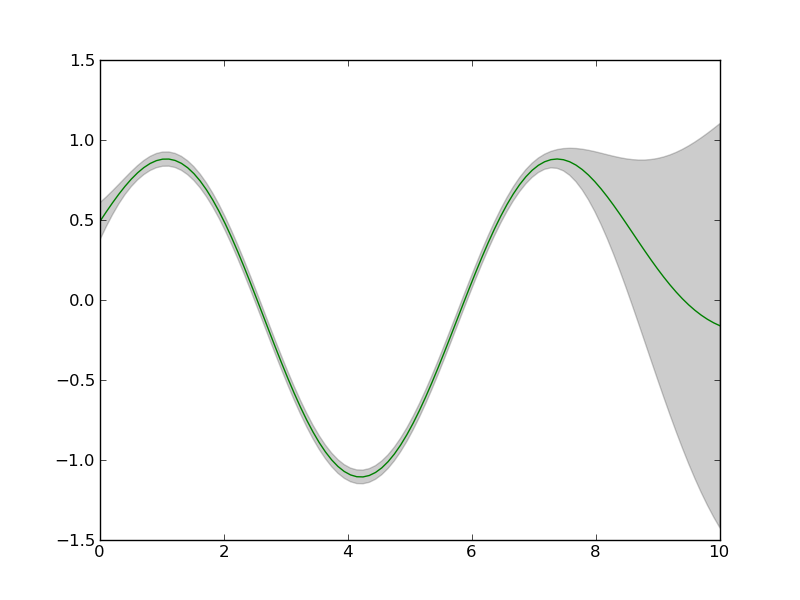
\includegraphics[height=8cm]{sausage.png}
\begin{description}
\item[{\textbf{returns:}}] \leavevmode{[}{[}fill\_plot, line\_plot{]}{]}
The fill and the line of the sausage plot. (i.e. green line and gray fill of the example above)

\end{description}

\textbf{Parameters:}
\begin{description}
\item[{X}] \leavevmode{[}{[}double{]}{]}
Interval X for which the saussage shall be plottet.

\item[{mean}] \leavevmode{[}{[}double{]}{]}
The mean of to be plottet.

\item[{std}] \leavevmode{[}{[}double{]}{]}
Pointwise standard deviation.

\item[{format\_fill}] \leavevmode{[}\{format\}{]}
The format of the fill. See \href{http://matplotlib.sourceforge.net/}{http://matplotlib.sourceforge.net/} for details.

\item[{format\_line}] \leavevmode{[}\{format\}{]}
The format of the mean line. See \href{http://matplotlib.sourceforge.net/}{http://matplotlib.sourceforge.net/} for details.

\end{description}

\end{fulllineitems}

\index{plot\_training\_data() (in module pygp.plot.gpr\_plot)}

\begin{fulllineitems}
\phantomsection\label{plot_gpr:pygp.plot.gpr_plot.plot_training_data}\pysiglinewithargsret{\code{pygp.plot.gpr\_plot.}\bfcode{plot\_training\_data}}{\emph{x}, \emph{y}, \emph{shift=None}, \emph{replicate\_indices=None}, \emph{format\_data=\{`marker': `.'}, \emph{`alpha': 0.5}, \emph{`markersize': 9}, \emph{`linestyle': `--`}, \emph{`lw': 1\}}, \emph{draw\_arrows=0}, \emph{plot\_old=False}}{}
Plot training data input x and output y into the
active figure (See \href{http://matplotlib.sourceforge.net/}{http://matplotlib.sourceforge.net/} for details of figure).

Instance plot without replicate groups:

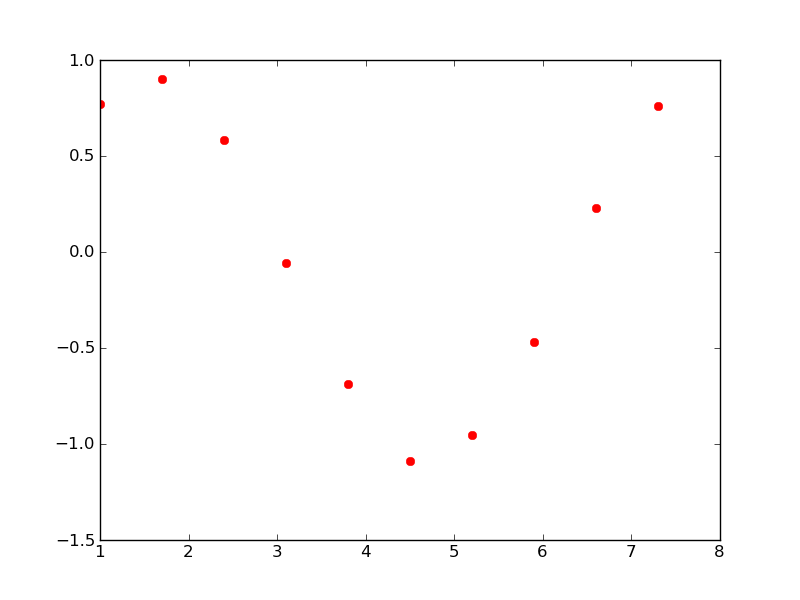
\includegraphics[height=8cm]{plotTraining.png}

Instance plot with two replicate groups and a shift in x-koords:

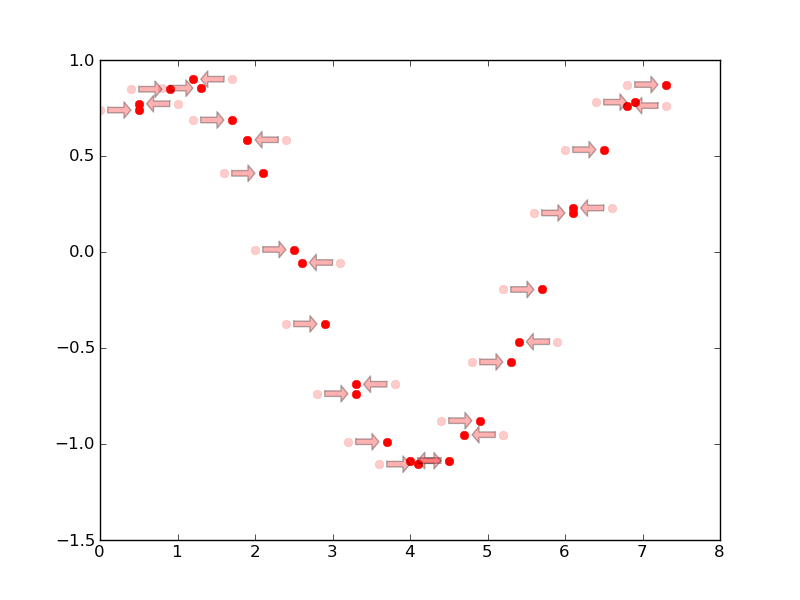
\includegraphics[height=8cm]{plotTrainingShiftX.png}

\textbf{Parameters:}
\begin{description}
\item[{x}] \leavevmode{[}{[}double{]}{]}
Input x (e.g. time).

\item[{y}] \leavevmode{[}{[}double{]}{]}
Output y (e.g. expression).

\item[{shift}] \leavevmode{[}{[}double{]}{]}
The shift of each replicate group.

\item[{replicate\_indices}] \leavevmode{[}{[}int{]}{]}
Indices of replicates for each x, rexpectively

\item[{format\_data}] \leavevmode{[}\{format\}{]}
Format of the data points. See \href{http://matplotlib.sourceforge.net/}{http://matplotlib.sourceforge.net/} for details.

\item[{draw\_arrows}] \leavevmode{[}int{]}
draw given number of arrows (if greator than len(replicate) draw all arrows.
Arrows will show the time shift for time points, respectively.

\end{description}

\end{fulllineitems}


See following examples for usage details:


\chapter{Application Example of GP regression}
\label{demo_gpr::doc}\label{demo_gpr:application-example-of-gp-regression}
This Example shows the Squared Exponential CF
(\code{covar.se.SEARDCF}) combined with noise
\code{covar.noise.NoiseISOCF} by summing them up
(using \code{covar.combinators.SumCF}).

First of all we have to import all important packages:

\begin{Verbatim}[commandchars=\\\{\}]
\PYG{k+kn}{import} \PYG{n+nn}{pylab} \PYG{k+kn}{as} \PYG{n+nn}{PL}
\PYG{k+kn}{import} \PYG{n+nn}{scipy} \PYG{k+kn}{as} \PYG{n+nn}{SP}
\PYG{k+kn}{import} \PYG{n+nn}{numpy.random} \PYG{k+kn}{as} \PYG{n+nn}{random}
\end{Verbatim}

Now import the Covariance Functions and Combinators:

\begin{Verbatim}[commandchars=\\\{\}]
\PYG{k+kn}{from} \PYG{n+nn}{pygp.covar} \PYG{k+kn}{import} \PYG{n}{se}\PYG{p}{,} \PYG{n}{noise}\PYG{p}{,} \PYG{n}{combinators}
\end{Verbatim}

And additionally the GP regression framework ({\hyperref[gp:module-pygp.gp]{\code{pygp.gp}}} and {\hyperref[priors:module-pygp.priors]{\code{pygp.priors}}} for the priors):

\begin{Verbatim}[commandchars=\\\{\}]
\PYG{k+kn}{from} \PYG{n+nn}{pygp.gp.basic\PYGZus{}gp} \PYG{k+kn}{import} \PYG{n}{GP}
\PYG{k+kn}{from} \PYG{n+nn}{pygp.optimize.optimize} \PYG{k+kn}{import} \PYG{n}{opt\PYGZus{}hyper}
\PYG{k+kn}{from} \PYG{n+nn}{pygp.priors} \PYG{k+kn}{import} \PYG{n}{lnpriors}
\PYG{k+kn}{import} \PYG{n+nn}{pygp.plot.gpr\PYGZus{}plot} \PYG{k+kn}{as} \PYG{n+nn}{gpr\PYGZus{}plot}
\end{Verbatim}

For this particular example we generate some simulated random sinus data, just samples from a superposition of a sin + linear trend:

\begin{Verbatim}[commandchars=\\\{\}]
\PYG{n}{random}\PYG{o}{.}\PYG{n}{seed}\PYG{p}{(}\PYG{l+m+mi}{1}\PYG{p}{)}
\PYG{n}{xmin} \PYG{o}{=} \PYG{l+m+mi}{1}
\PYG{n}{xmax} \PYG{o}{=} \PYG{l+m+mf}{2.5}\PYG{o}{*}\PYG{n}{SP}\PYG{o}{.}\PYG{n}{pi}
\PYG{n}{x} \PYG{o}{=} \PYG{n}{SP}\PYG{o}{.}\PYG{n}{arange}\PYG{p}{(}\PYG{n}{xmin}\PYG{p}{,}\PYG{n}{xmax}\PYG{p}{,}\PYG{l+m+mf}{0.7}\PYG{p}{)}

\PYG{n}{C} \PYG{o}{=} \PYG{l+m+mi}{2}       \PYG{c}{\PYGZsh{}offset}
\PYG{n}{b} \PYG{o}{=} \PYG{l+m+mf}{0.5}
\PYG{n}{sigma} \PYG{o}{=} \PYG{l+m+mf}{0.01}

\PYG{n}{b} \PYG{o}{=} \PYG{l+m+mi}{0}

\PYG{n}{y}  \PYG{o}{=} \PYG{n}{b}\PYG{o}{*}\PYG{n}{x} \PYG{o}{+} \PYG{n}{C} \PYG{o}{+} \PYG{l+m+mi}{1}\PYG{o}{*}\PYG{n}{SP}\PYG{o}{.}\PYG{n}{sin}\PYG{p}{(}\PYG{n}{x}\PYG{p}{)}
\PYG{n}{dy} \PYG{o}{=} \PYG{n}{b}   \PYG{o}{+}     \PYG{l+m+mi}{1}\PYG{o}{*}\PYG{n}{SP}\PYG{o}{.}\PYG{n}{cos}\PYG{p}{(}\PYG{n}{x}\PYG{p}{)}
\PYG{n}{y} \PYG{o}{+}\PYG{o}{=} \PYG{n}{sigma}\PYG{o}{*}\PYG{n}{random}\PYG{o}{.}\PYG{n}{randn}\PYG{p}{(}\PYG{n}{y}\PYG{o}{.}\PYG{n}{shape}\PYG{p}{[}\PYG{l+m+mi}{0}\PYG{p}{]}\PYG{p}{)}

\PYG{n}{y}\PYG{o}{-}\PYG{o}{=} \PYG{n}{y}\PYG{o}{.}\PYG{n}{mean}\PYG{p}{(}\PYG{p}{)}

\PYG{n}{x} \PYG{o}{=} \PYG{n}{x}\PYG{p}{[}\PYG{p}{:}\PYG{p}{,}\PYG{n}{SP}\PYG{o}{.}\PYG{n}{newaxis}\PYG{p}{]}
\end{Verbatim}

The predictions we will make on the interpolation interval

\begin{Verbatim}[commandchars=\\\{\}]
\PYG{n}{X} \PYG{o}{=} \PYG{n}{SP}\PYG{o}{.}\PYG{n}{linspace}\PYG{p}{(}\PYG{l+m+mi}{0}\PYG{p}{,}\PYG{l+m+mi}{10}\PYG{p}{,}\PYG{l+m+mi}{100}\PYG{p}{)}\PYG{p}{[}\PYG{p}{:}\PYG{p}{,}\PYG{n}{SP}\PYG{o}{.}\PYG{n}{newaxis}\PYG{p}{]}
\end{Verbatim}

Our starting hyperparameters are:

\begin{Verbatim}[commandchars=\\\{\}]
\PYG{n}{dim} \PYG{o}{=} \PYG{l+m+mi}{1}
\PYG{n}{logthetaCOVAR} \PYG{o}{=} \PYG{n}{SP}\PYG{o}{.}\PYG{n}{log}\PYG{p}{(}\PYG{p}{[}\PYG{l+m+mi}{1}\PYG{p}{,}\PYG{l+m+mi}{1}\PYG{p}{,}\PYG{n}{sigma}\PYG{p}{]}\PYG{p}{)}
\PYG{n}{hyperparams} \PYG{o}{=} \PYG{p}{\PYGZob{}}\PYG{l+s}{'}\PYG{l+s}{covar}\PYG{l+s}{'}\PYG{p}{:}\PYG{n}{logthetaCOVAR}\PYG{p}{\PYGZcb{}}
\end{Verbatim}

Now the interesting point: creating the sumCF by combining noise and se:

\begin{Verbatim}[commandchars=\\\{\}]
\PYG{n}{SECF} \PYG{o}{=} \PYG{n}{se}\PYG{o}{.}\PYG{n}{SEARDCF}\PYG{p}{(}\PYG{n}{dim}\PYG{p}{)}
\PYG{n}{noiseCF} \PYG{o}{=} \PYG{n}{noise}\PYG{o}{.}\PYG{n}{NoiseISOCF}\PYG{p}{(}\PYG{p}{)}
\PYG{n}{covar} \PYG{o}{=} \PYG{n}{combinators}\PYG{o}{.}\PYG{n}{SumCF}\PYG{p}{(}\PYG{p}{(}\PYG{n}{SECF}\PYG{p}{,}\PYG{n}{noiseCF}\PYG{p}{)}\PYG{p}{)}
\end{Verbatim}

And the prior believes, we have about the hyperparameters:

\begin{Verbatim}[commandchars=\\\{\}]
\PYG{c}{\PYGZsh{}Length-Scale}
\PYG{n}{covar\PYGZus{}priors} \PYG{o}{=} \PYG{p}{[}\PYG{p}{]}
\PYG{n}{covar\PYGZus{}priors}\PYG{o}{.}\PYG{n}{append}\PYG{p}{(}\PYG{p}{[}\PYG{n}{lnpriors}\PYG{o}{.}\PYG{n}{lngammapdf}\PYG{p}{,}\PYG{p}{[}\PYG{l+m+mi}{1}\PYG{p}{,}\PYG{l+m+mi}{2}\PYG{p}{]}\PYG{p}{]}\PYG{p}{)}
\PYG{k}{for} \PYG{n}{i} \PYG{o+ow}{in} \PYG{n+nb}{range}\PYG{p}{(}\PYG{n}{dim}\PYG{p}{)}\PYG{p}{:}
    \PYG{n}{covar\PYGZus{}priors}\PYG{o}{.}\PYG{n}{append}\PYG{p}{(}\PYG{p}{[}\PYG{n}{lnpriors}\PYG{o}{.}\PYG{n}{lngammapdf}\PYG{p}{,}\PYG{p}{[}\PYG{l+m+mi}{1}\PYG{p}{,}\PYG{l+m+mi}{1}\PYG{p}{]}\PYG{p}{]}\PYG{p}{)}
\PYG{c}{\PYGZsh{}Noise}
\PYG{n}{covar\PYGZus{}priors}\PYG{o}{.}\PYG{n}{append}\PYG{p}{(}\PYG{p}{[}\PYG{n}{lnpriors}\PYG{o}{.}\PYG{n}{lngammapdf}\PYG{p}{,}\PYG{p}{[}\PYG{l+m+mi}{1}\PYG{p}{,}\PYG{l+m+mi}{1}\PYG{p}{]}\PYG{p}{]}\PYG{p}{)}
\PYG{n}{priors} \PYG{o}{=} \PYG{p}{\PYGZob{}}\PYG{l+s}{'}\PYG{l+s}{covar}\PYG{l+s}{'}\PYG{p}{:}\PYG{n}{covar\PYGZus{}priors}\PYG{p}{\PYGZcb{}}
\end{Verbatim}

We do want all hyperparameter to be optimized:

\begin{Verbatim}[commandchars=\\\{\}]
\PYG{n}{Ifilter} \PYG{o}{=} \PYG{p}{\PYGZob{}}\PYG{l+s}{'}\PYG{l+s}{covar}\PYG{l+s}{'}\PYG{p}{:} \PYG{n}{SP}\PYG{o}{.}\PYG{n}{array}\PYG{p}{(}\PYG{p}{[}\PYG{l+m+mi}{1}\PYG{p}{,}\PYG{l+m+mi}{1}\PYG{p}{,}\PYG{l+m+mi}{1}\PYG{p}{]}\PYG{p}{,}\PYG{n}{dtype}\PYG{o}{=}\PYG{l+s}{'}\PYG{l+s}{int}\PYG{l+s}{'}\PYG{p}{)}\PYG{p}{\PYGZcb{}}
\end{Verbatim}

Create the GP regression class for further usage:

\begin{Verbatim}[commandchars=\\\{\}]
\PYG{n}{gpr} \PYG{o}{=} \PYG{n}{GP}\PYG{p}{(}\PYG{n}{covar}\PYG{p}{,}\PYG{n}{x}\PYG{o}{=}\PYG{n}{x}\PYG{p}{,}\PYG{n}{y}\PYG{o}{=}\PYG{n}{y}\PYG{p}{)}
\end{Verbatim}

And optimize the hyperparameters:

\begin{Verbatim}[commandchars=\\\{\}]
\PYG{p}{[}\PYG{n}{opt\PYGZus{}model\PYGZus{}params}\PYG{p}{,}\PYG{n}{opt\PYGZus{}lml}\PYG{p}{]}\PYG{o}{=} \PYG{n}{opt\PYGZus{}hyper}\PYG{p}{(}\PYG{n}{gpr}\PYG{p}{,}\PYG{n}{hyperparams}\PYG{p}{,}\PYG{n}{priors}\PYG{o}{=}\PYG{n}{priors}\PYG{p}{,}\PYG{n}{gradcheck}\PYG{o}{=}\PYG{n+nb+bp}{True}\PYG{p}{,}\PYG{n}{Ifilter}\PYG{o}{=}\PYG{n}{Ifilter}\PYG{p}{)}
\end{Verbatim}

With these optimized hyperparameters we can now predict the point-wise mean and deviance of the training data:

\begin{Verbatim}[commandchars=\\\{\}]
\PYG{p}{[}\PYG{n}{M}\PYG{p}{,}\PYG{n}{S}\PYG{p}{]} \PYG{o}{=} \PYG{n}{gpr}\PYG{o}{.}\PYG{n}{predict}\PYG{p}{(}\PYG{n}{opt\PYGZus{}model\PYGZus{}params}\PYG{p}{,}\PYG{n}{X}\PYG{p}{)}
\end{Verbatim}

For the sake of beauty plot the mean and deviance:

\begin{Verbatim}[commandchars=\\\{\}]
\PYG{n}{gpr\PYGZus{}plot}\PYG{o}{.}\PYG{n}{plot\PYGZus{}sausage}\PYG{p}{(}\PYG{n}{X}\PYG{p}{,}\PYG{n}{M}\PYG{p}{,}\PYG{n}{SP}\PYG{o}{.}\PYG{n}{sqrt}\PYG{p}{(}\PYG{n}{S}\PYG{p}{)}\PYG{p}{)}
\PYG{n}{gpr\PYGZus{}plot}\PYG{o}{.}\PYG{n}{plot\PYGZus{}training\PYGZus{}data}\PYG{p}{(}\PYG{n}{x}\PYG{p}{,}\PYG{n}{y}\PYG{p}{)}
\end{Verbatim}

The resulting plot is:

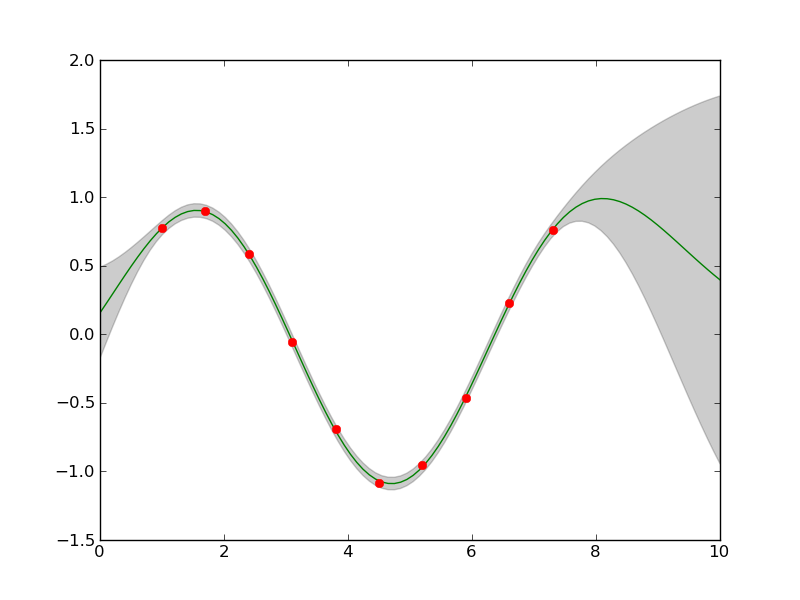
\includegraphics{gprExample.png}


\chapter{Application Example of GP regression}
\label{demo_gpr_shiftx::doc}\label{demo_gpr_shiftx:application-example-of-gp-regression}
This Example shows the Squared Exponential CF
(\code{pygp.covar.se.SEARDCF}) preprocessed by
shiftCF(:py:class{}`covar.combinators.ShiftCF) and combined with noise
\code{pygp.covar.noise.NoiseISOCF} by summing them up
(using {\hyperref[covars:pygp.covar.combinators.SumCF]{\code{pygp.covar.combinators.SumCF}}}).
We will shift two input replicates against each other, to make them fit to each other.

First of all we have to import all important packages:

\begin{Verbatim}[commandchars=\\\{\}]
\PYG{k+kn}{import} \PYG{n+nn}{pylab} \PYG{k+kn}{as} \PYG{n+nn}{PL}
\PYG{k+kn}{import} \PYG{n+nn}{scipy} \PYG{k+kn}{as} \PYG{n+nn}{SP}
\PYG{k+kn}{import} \PYG{n+nn}{numpy.random} \PYG{k+kn}{as} \PYG{n+nn}{random}
\end{Verbatim}

Now import the Covariance Functions and Combinators:

\begin{Verbatim}[commandchars=\\\{\}]
\PYG{k+kn}{from} \PYG{n+nn}{pygp.covar} \PYG{k+kn}{import} \PYG{n}{se}\PYG{p}{,} \PYG{n}{noise}\PYG{p}{,} \PYG{n}{combinators}
\end{Verbatim}

And additionally the GP regression framework ({\hyperref[gp:module-pygp.gp]{\code{pygp.gp}}}, {\hyperref[priors:module-pygp.priors]{\code{pygp.priors}}} for the priors and {\hyperref[plot_gpr:module-pygp.plot.gpr_plot]{\code{pygp.plot.gpr\_plot}}} for plotting the results):

\begin{Verbatim}[commandchars=\\\{\}]
\PYG{k+kn}{from} \PYG{n+nn}{pygp.gp.basic\PYGZus{}gp} \PYG{k+kn}{import} \PYG{n}{GP}
\PYG{k+kn}{from} \PYG{n+nn}{pygp.optimize.optimize} \PYG{k+kn}{import} \PYG{n}{opt\PYGZus{}hyper}
\PYG{k+kn}{from} \PYG{n+nn}{pygp.priors} \PYG{k+kn}{import} \PYG{n}{lnpriors}
\PYG{k+kn}{import} \PYG{n+nn}{pygp.plot.gpr\PYGZus{}plot} \PYG{k+kn}{as} \PYG{n+nn}{gpr\PYGZus{}plot}
\end{Verbatim}

For this particular example we generate some simulated random sinus
data; just samples from a superposition of a \emph{sin + linear} trend:

\begin{Verbatim}[commandchars=\\\{\}]
\PYG{n}{xmin} \PYG{o}{=} \PYG{l+m+mi}{1}
\PYG{n}{xmax} \PYG{o}{=} \PYG{l+m+mf}{2.5}\PYG{o}{*}\PYG{n}{SP}\PYG{o}{.}\PYG{n}{pi}
\PYG{n}{x1} \PYG{o}{=} \PYG{n}{SP}\PYG{o}{.}\PYG{n}{arange}\PYG{p}{(}\PYG{n}{xmin}\PYG{p}{,}\PYG{n}{xmax}\PYG{p}{,}\PYG{o}{.}\PYG{l+m+mi}{7}\PYG{p}{)}
\PYG{n}{x2} \PYG{o}{=} \PYG{n}{SP}\PYG{o}{.}\PYG{n}{arange}\PYG{p}{(}\PYG{n}{xmin}\PYG{p}{,}\PYG{n}{xmax}\PYG{p}{,}\PYG{o}{.}\PYG{l+m+mi}{4}\PYG{p}{)}

\PYG{n}{C} \PYG{o}{=} \PYG{l+m+mi}{2}       \PYG{c}{\PYGZsh{}offset}
\PYG{n}{b} \PYG{o}{=} \PYG{l+m+mf}{0.5}
\PYG{n}{sigma} \PYG{o}{=} \PYG{l+m+mf}{0.1}

\PYG{n}{b} \PYG{o}{=} \PYG{l+m+mi}{0}

\PYG{n}{y1}  \PYG{o}{=} \PYG{n}{b}\PYG{o}{*}\PYG{n}{x1} \PYG{o}{+} \PYG{n}{C} \PYG{o}{+} \PYG{l+m+mi}{1}\PYG{o}{*}\PYG{n}{SP}\PYG{o}{.}\PYG{n}{sin}\PYG{p}{(}\PYG{n}{x1}\PYG{p}{)}
\PYG{n}{dy1} \PYG{o}{=} \PYG{n}{b}   \PYG{o}{+}     \PYG{l+m+mi}{1}\PYG{o}{*}\PYG{n}{SP}\PYG{o}{.}\PYG{n}{cos}\PYG{p}{(}\PYG{n}{x1}\PYG{p}{)}
\PYG{n}{y1} \PYG{o}{+}\PYG{o}{=} \PYG{n}{sigma}\PYG{o}{*}\PYG{n}{random}\PYG{o}{.}\PYG{n}{randn}\PYG{p}{(}\PYG{n}{y1}\PYG{o}{.}\PYG{n}{shape}\PYG{p}{[}\PYG{l+m+mi}{0}\PYG{p}{]}\PYG{p}{)}
\PYG{n}{y1}\PYG{o}{-}\PYG{o}{=} \PYG{n}{y1}\PYG{o}{.}\PYG{n}{mean}\PYG{p}{(}\PYG{p}{)}

\PYG{n}{y2}  \PYG{o}{=} \PYG{n}{b}\PYG{o}{*}\PYG{n}{x2} \PYG{o}{+} \PYG{n}{C} \PYG{o}{+} \PYG{l+m+mi}{1}\PYG{o}{*}\PYG{n}{SP}\PYG{o}{.}\PYG{n}{sin}\PYG{p}{(}\PYG{n}{x2}\PYG{p}{)}
\PYG{n}{dy2} \PYG{o}{=} \PYG{n}{b}   \PYG{o}{+}     \PYG{l+m+mi}{1}\PYG{o}{*}\PYG{n}{SP}\PYG{o}{.}\PYG{n}{cos}\PYG{p}{(}\PYG{n}{x2}\PYG{p}{)}
\PYG{n}{y2} \PYG{o}{+}\PYG{o}{=} \PYG{n}{sigma}\PYG{o}{*}\PYG{n}{random}\PYG{o}{.}\PYG{n}{randn}\PYG{p}{(}\PYG{n}{y2}\PYG{o}{.}\PYG{n}{shape}\PYG{p}{[}\PYG{l+m+mi}{0}\PYG{p}{]}\PYG{p}{)}
\PYG{n}{y2}\PYG{o}{-}\PYG{o}{=} \PYG{n}{y2}\PYG{o}{.}\PYG{n}{mean}\PYG{p}{(}\PYG{p}{)}

\PYG{n}{x1} \PYG{o}{=} \PYG{n}{x1}\PYG{p}{[}\PYG{p}{:}\PYG{p}{,}\PYG{n}{SP}\PYG{o}{.}\PYG{n}{newaxis}\PYG{p}{]}
\PYG{n}{x2} \PYG{o}{=} \PYG{p}{(}\PYG{n}{x2}\PYG{o}{-}\PYG{l+m+mi}{1}\PYG{p}{)}\PYG{p}{[}\PYG{p}{:}\PYG{p}{,}\PYG{n}{SP}\PYG{o}{.}\PYG{n}{newaxis}\PYG{p}{]}

\PYG{n}{x} \PYG{o}{=} \PYG{n}{SP}\PYG{o}{.}\PYG{n}{concatenate}\PYG{p}{(}\PYG{p}{(}\PYG{n}{x1}\PYG{p}{,}\PYG{n}{x2}\PYG{p}{)}\PYG{p}{,}\PYG{n}{axis}\PYG{o}{=}\PYG{l+m+mi}{0}\PYG{p}{)}
\PYG{n}{y} \PYG{o}{=} \PYG{n}{SP}\PYG{o}{.}\PYG{n}{concatenate}\PYG{p}{(}\PYG{p}{(}\PYG{n}{y1}\PYG{p}{,}\PYG{n}{y2}\PYG{p}{)}\PYG{p}{,}\PYG{n}{axis}\PYG{o}{=}\PYG{l+m+mi}{0}\PYG{p}{)}
\end{Verbatim}

The predictions we will make on the interpolation interval

\begin{Verbatim}[commandchars=\\\{\}]
\PYG{n}{X} \PYG{o}{=} \PYG{n}{SP}\PYG{o}{.}\PYG{n}{linspace}\PYG{p}{(}\PYG{o}{-}\PYG{l+m+mi}{2}\PYG{p}{,}\PYG{l+m+mi}{10}\PYG{p}{,}\PYG{l+m+mi}{100}\PYG{p}{)}\PYG{p}{[}\PYG{p}{:}\PYG{p}{,}\PYG{n}{SP}\PYG{o}{.}\PYG{n}{newaxis}\PYG{p}{]}
\end{Verbatim}

For the calculation of the replicates, we need to give the replicate indices per input x:

\begin{Verbatim}[commandchars=\\\{\}]
\PYG{n}{dim} \PYG{o}{=} \PYG{l+m+mi}{1}
\PYG{n}{replicate\PYGZus{}indices} \PYG{o}{=} \PYG{n}{SP}\PYG{o}{.}\PYG{n}{concatenate}\PYG{p}{(}\PYG{p}{[}\PYG{n}{SP}\PYG{o}{.}\PYG{n}{repeat}\PYG{p}{(}\PYG{n}{i}\PYG{p}{,}\PYG{n+nb}{len}\PYG{p}{(}\PYG{n}{xi}\PYG{p}{)}\PYG{p}{)} \PYG{k}{for} \PYG{n}{i}\PYG{p}{,}\PYG{n}{xi} \PYG{o+ow}{in} \PYG{n+nb}{enumerate}\PYG{p}{(}\PYG{p}{(}\PYG{n}{x1}\PYG{p}{,}\PYG{n}{x2}\PYG{p}{)}\PYG{p}{)}\PYG{p}{]}\PYG{p}{)}
\PYG{n}{n\PYGZus{}replicates} \PYG{o}{=} \PYG{n+nb}{len}\PYG{p}{(}\PYG{n}{SP}\PYG{o}{.}\PYG{n}{unique}\PYG{p}{(}\PYG{n}{replicate\PYGZus{}indices}\PYG{p}{)}\PYG{p}{)}
\end{Verbatim}

Thus, our starting hyperparameters are:

\begin{Verbatim}[commandchars=\\\{\}]
\PYG{n}{logthetaCOVAR} \PYG{o}{=} \PYG{n}{SP}\PYG{o}{.}\PYG{n}{log}\PYG{p}{(}\PYG{p}{[}\PYG{l+m+mi}{1}\PYG{p}{,}\PYG{l+m+mi}{1}\PYG{p}{,}\PYG{l+m+mi}{1}\PYG{p}{,}\PYG{l+m+mi}{1}\PYG{p}{,}\PYG{n}{sigma}\PYG{p}{]}\PYG{p}{)}
\PYG{n}{hyperparams} \PYG{o}{=} \PYG{p}{\PYGZob{}}\PYG{l+s}{'}\PYG{l+s}{covar}\PYG{l+s}{'}\PYG{p}{:}\PYG{n}{logthetaCOVAR}\PYG{p}{\PYGZcb{}}
\end{Verbatim}

Now the interesting point: creating the sumCF by combining noise and se:

\begin{Verbatim}[commandchars=\\\{\}]
\PYG{n}{SECF} \PYG{o}{=} \PYG{n}{se}\PYG{o}{.}\PYG{n}{SEARDCF}\PYG{p}{(}\PYG{n}{dim}\PYG{p}{)}
\PYG{n}{noiseCF} \PYG{o}{=} \PYG{n}{noise}\PYG{o}{.}\PYG{n}{NoiseISOCF}\PYG{p}{(}\PYG{p}{)}
\PYG{n}{shiftCF} \PYG{o}{=} \PYG{n}{combinators}\PYG{o}{.}\PYG{n}{ShiftCF}\PYG{p}{(}\PYG{n}{SECF}\PYG{p}{,}\PYG{n}{replicate\PYGZus{}indices}\PYG{p}{)}
\PYG{n}{covar} \PYG{o}{=} \PYG{n}{combinators}\PYG{o}{.}\PYG{n}{SumCF}\PYG{p}{(}\PYG{p}{(}\PYG{n}{shiftCF}\PYG{p}{,}\PYG{n}{noiseCF}\PYG{p}{)}\PYG{p}{)}
\end{Verbatim}

And the prior believes, we have about the hyperparameters:

\begin{Verbatim}[commandchars=\\\{\}]
\PYG{n}{covar\PYGZus{}priors} \PYG{o}{=} \PYG{p}{[}\PYG{p}{]}
\PYG{c}{\PYGZsh{}Length-Scale}
\PYG{n}{covar\PYGZus{}priors}\PYG{o}{.}\PYG{n}{append}\PYG{p}{(}\PYG{p}{[}\PYG{n}{lnpriors}\PYG{o}{.}\PYG{n}{lngammapdf}\PYG{p}{,}\PYG{p}{[}\PYG{l+m+mi}{1}\PYG{p}{,}\PYG{l+m+mi}{2}\PYG{p}{]}\PYG{p}{]}\PYG{p}{)}
\PYG{k}{for} \PYG{n}{i} \PYG{o+ow}{in} \PYG{n+nb}{range}\PYG{p}{(}\PYG{n}{dim}\PYG{p}{)}\PYG{p}{:}
    \PYG{n}{covar\PYGZus{}priors}\PYG{o}{.}\PYG{n}{append}\PYG{p}{(}\PYG{p}{[}\PYG{n}{lnpriors}\PYG{o}{.}\PYG{n}{lngammapdf}\PYG{p}{,}\PYG{p}{[}\PYG{l+m+mi}{1}\PYG{p}{,}\PYG{l+m+mi}{1}\PYG{p}{]}\PYG{p}{]}\PYG{p}{)}

\PYG{c}{\PYGZsh{}X-Shift}
\PYG{k}{for} \PYG{n}{i} \PYG{o+ow}{in} \PYG{n+nb}{range}\PYG{p}{(}\PYG{n}{n\PYGZus{}replicates}\PYG{p}{)}\PYG{p}{:}
    \PYG{n}{covar\PYGZus{}priors}\PYG{o}{.}\PYG{n}{append}\PYG{p}{(}\PYG{p}{[}\PYG{n}{lnpriors}\PYG{o}{.}\PYG{n}{lngausspdf}\PYG{p}{,}\PYG{p}{[}\PYG{l+m+mi}{0}\PYG{p}{,}\PYG{o}{.}\PYG{l+m+mi}{5}\PYG{p}{]}\PYG{p}{]}\PYG{p}{)}

\PYG{c}{\PYGZsh{}Noise}
\PYG{n}{covar\PYGZus{}priors}\PYG{o}{.}\PYG{n}{append}\PYG{p}{(}\PYG{p}{[}\PYG{n}{lnpriors}\PYG{o}{.}\PYG{n}{lngammapdf}\PYG{p}{,}\PYG{p}{[}\PYG{l+m+mi}{1}\PYG{p}{,}\PYG{l+m+mi}{1}\PYG{p}{]}\PYG{p}{]}\PYG{p}{)}
\PYG{n}{priors} \PYG{o}{=} \PYG{p}{\PYGZob{}}\PYG{l+s}{'}\PYG{l+s}{covar}\PYG{l+s}{'}\PYG{p}{:}\PYG{n}{covar\PYGZus{}priors}\PYG{p}{\PYGZcb{}}
\end{Verbatim}

We want all hyperparameters to be optimized:

\begin{Verbatim}[commandchars=\\\{\}]
\PYG{n}{Ifilter} \PYG{o}{=} \PYG{p}{\PYGZob{}}\PYG{l+s}{'}\PYG{l+s}{covar}\PYG{l+s}{'}\PYG{p}{:} \PYG{n}{SP}\PYG{o}{.}\PYG{n}{array}\PYG{p}{(}\PYG{p}{[}\PYG{l+m+mi}{1}\PYG{p}{,}\PYG{l+m+mi}{1}\PYG{p}{,}\PYG{l+m+mi}{1}\PYG{p}{,}\PYG{l+m+mi}{1}\PYG{p}{,}\PYG{l+m+mi}{1}\PYG{p}{]}\PYG{p}{,}\PYG{n}{dtype}\PYG{o}{=}\PYG{l+s}{'}\PYG{l+s}{int}\PYG{l+s}{'}\PYG{p}{)}\PYG{p}{\PYGZcb{}}
\end{Verbatim}

Create the GP regression class for further usage:

\begin{Verbatim}[commandchars=\\\{\}]
\PYG{n}{gpr} \PYG{o}{=} \PYG{n}{GP}\PYG{p}{(}\PYG{n}{covar}\PYG{p}{,}\PYG{n}{x}\PYG{o}{=}\PYG{n}{x}\PYG{p}{,}\PYG{n}{y}\PYG{o}{=}\PYG{n}{y}\PYG{p}{)}
\end{Verbatim}

And optimize the hyperparameters:

\begin{Verbatim}[commandchars=\\\{\}]
\PYG{p}{[}\PYG{n}{opt\PYGZus{}model\PYGZus{}params}\PYG{p}{,}\PYG{n}{opt\PYGZus{}lml}\PYG{p}{]}\PYG{o}{=}\PYG{n}{opt\PYGZus{}hyper}\PYG{p}{(}\PYG{n}{gpr}\PYG{p}{,}\PYG{n}{hyperparams}\PYG{p}{,}\PYG{n}{priors}\PYG{o}{=}\PYG{n}{priors}\PYG{p}{,}\PYG{n}{gradcheck}\PYG{o}{=}\PYG{n+nb+bp}{True}\PYG{p}{,}\PYG{n}{Ifilter}\PYG{o}{=}\PYG{n}{Ifilter}\PYG{p}{)}
\end{Verbatim}

With these optimized hyperparameters we can now predict the point-wise mean M and deviance S of the training data:

\begin{Verbatim}[commandchars=\\\{\}]
\PYG{p}{[}\PYG{n}{M}\PYG{p}{,}\PYG{n}{S}\PYG{p}{]} \PYG{o}{=} \PYG{n}{gpr}\PYG{o}{.}\PYG{n}{predict}\PYG{p}{(}\PYG{n}{opt\PYGZus{}model\PYGZus{}params}\PYG{p}{,}\PYG{n}{X}\PYG{p}{)}
\end{Verbatim}

For the sake of beauty plot the mean M and deviance S:

\begin{Verbatim}[commandchars=\\\{\}]
\PYG{n}{T} \PYG{o}{=} \PYG{n}{opt\PYGZus{}model\PYGZus{}params}\PYG{p}{[}\PYG{l+s}{'}\PYG{l+s}{covar}\PYG{l+s}{'}\PYG{p}{]}\PYG{p}{[}\PYG{l+m+mi}{2}\PYG{p}{:}\PYG{l+m+mi}{4}\PYG{p}{]}
\PYG{n}{gpr\PYGZus{}plot}\PYG{o}{.}\PYG{n}{plot\PYGZus{}sausage}\PYG{p}{(}\PYG{n}{X}\PYG{p}{,}\PYG{n}{M}\PYG{p}{,}\PYG{n}{SP}\PYG{o}{.}\PYG{n}{sqrt}\PYG{p}{(}\PYG{n}{S}\PYG{p}{)}\PYG{p}{)}
\PYG{n}{gpr\PYGZus{}plot}\PYG{o}{.}\PYG{n}{plot\PYGZus{}training\PYGZus{}data}\PYG{p}{(}\PYG{n}{x}\PYG{p}{,}\PYG{n}{y}\PYG{p}{,}\PYG{n}{shift}\PYG{o}{=}\PYG{n}{T}\PYG{p}{,}\PYG{n}{replicate\PYGZus{}indices}\PYG{o}{=}\PYG{n}{replicate\PYGZus{}indices}\PYG{p}{)}
\end{Verbatim}

The resulting plot is:

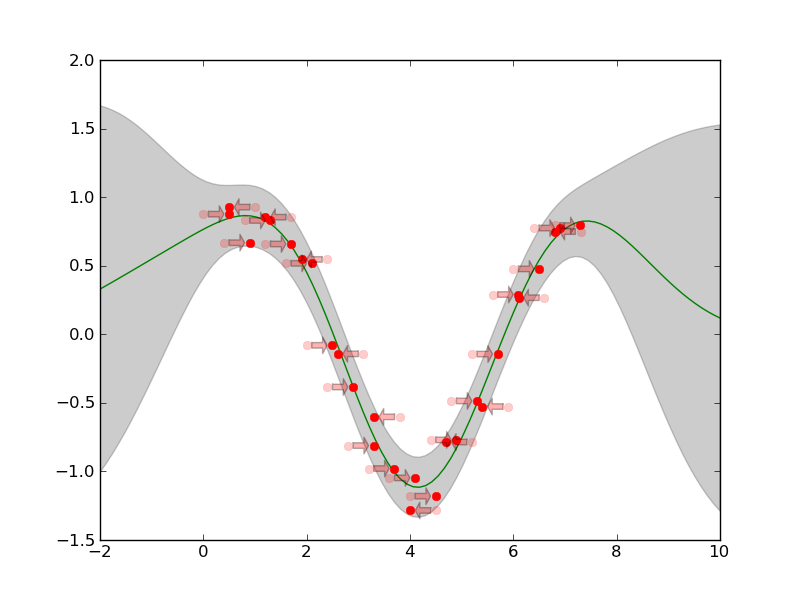
\includegraphics{TimeShiftExample.png}


\chapter{Indices and tables}
\label{index:indices-and-tables}\begin{itemize}
\item {} 
\emph{genindex}

\item {} 
\emph{modindex}

\item {} 
\emph{search}

\end{itemize}


\renewcommand{\indexname}{Python Module Index}
\begin{theindex}
\def\bigletter#1{{\Large\sffamily#1}\nopagebreak\vspace{1mm}}
\bigletter{p}
\item {\texttt{pygp.covar}}, \pageref{covars:module-pygp.covar}
\item {\texttt{pygp.covar.combinators}}, \pageref{covars:module-pygp.covar.combinators}
\item {\texttt{pygp.covar.fixed}}, \pageref{covars:module-pygp.covar.fixed}
\item {\texttt{pygp.covar.linear}}, \pageref{covars:module-pygp.covar.linear}
\item {\texttt{pygp.covar.noise}}, \pageref{covars:module-pygp.covar.noise}
\item {\texttt{pygp.covar.se}}, \pageref{covars:module-pygp.covar.se}
\item {\texttt{pygp.gp}}, \pageref{gp:module-pygp.gp}
\item {\texttt{pygp.gp.composite}}, \pageref{gp:module-pygp.gp.composite}
\item {\texttt{pygp.gp.gp\_base}}, \pageref{gp:module-pygp.gp.gp_base}
\item {\texttt{pygp.gp.gpcEP}}, \pageref{gp:module-pygp.gp.gpcEP}
\item {\texttt{pygp.gp.gplvm}}, \pageref{gp:module-pygp.gp.gplvm}
\item {\texttt{pygp.gp.gprEP}}, \pageref{gp:module-pygp.gp.gprEP}
\item {\texttt{pygp.optimize}}, \pageref{opt_hyper:module-pygp.optimize}
\item {\texttt{pygp.optimize.optimize\_base}}, \pageref{opt_hyper:module-pygp.optimize.optimize_base}
\item {\texttt{pygp.plot}}, \pageref{plot_gpr:module-pygp.plot}
\item {\texttt{pygp.plot.gpr\_plot}}, \pageref{plot_gpr:module-pygp.plot.gpr_plot}
\item {\texttt{pygp.priors}}, \pageref{priors:module-pygp.priors}
\item {\texttt{pygp.priors.lnpriors}}, \pageref{priors:module-pygp.priors.lnpriors}
\end{theindex}

\renewcommand{\indexname}{Index}
\printindex
\end{document}
